\PassOptionsToPackage{utf8}{inputenc}
\documentclass{bioinfo}

\usepackage[draft]{hyperref}
\hypersetup{colorlinks=true,urlcolor=black,linkcolor=black,citecolor=black}
\usepackage{makecell}
\usepackage{comment}

\usepackage{floatrow}

% singlelinecheck=false puts subcaptions on the left
\usepackage[singlelinecheck=false]{subcaption}

\usepackage{algorithm2e}
\usepackage[usenames,dvipsnames]{xcolor}

\usepackage{orcidlink}
\usepackage{paralist}

\usepackage{amsmath}

\usepackage{cleveref}

% table stuff
\usepackage{amsfonts}
\usepackage{booktabs}
\usepackage{siunitx}
\newcommand{\ra}[1]{\renewcommand{\arraystretch}{#1}}
\usepackage{float}
\floatstyle{plaintop}
\restylefloat{table}

% we squeeze our figures even more together
\captionsetup{belowskip=-2pt}

\SetAlgoLined
\SetKwProg{MyStruct}{Struct}{ contains}{end}

\newcommand{\vocab}{\textbf}
\newcommand{\red}[1]{{\textcolor{Red}{#1}}}
\newcommand{\FIXME}[1]{\red{[FIXME: #1]}}
\newcommand{\REVIEWED}[1]{{\textcolor{Black}{#1}}}
\newcommand{\beginsupplement}{%
    \renewcommand{\thesection}{S}
	\setcounter{table}{0}
	\renewcommand{\thetable}{S\arabic{table}}%
	\setcounter{figure}{0}
	\renewcommand{\thefigure}{S\arabic{figure}}%
}

\def\labelitemi{--}

\copyrightyear{2022} \pubyear{XXXX}

\access{Advance Access Publication Date: Day Month Year}
\appnotes{Genome Analysis}

\begin{document}
\firstpage{1}

\subtitle{Genome Analysis}

\title[ODGI: understanding pangenome graphs]{ODGI: understanding pangenome graphs}
\author[Guarracino, Heumos \textit{et~al}.]{
Andrea~Guarracino\orcidlink{0000-0001-9744-131X}\,$^{\text{\sfb 1} \dagger}$,
Simon~Heumos\orcidlink{0000-0003-3326-817X},$^{\text{\sfb 2,3} \dagger}$
Sven~Nahnsen\orcidlink{0000-0002-4375-0691}$^{\text{\sfb 2,3}}$, \\
Pjotr~Prins\orcidlink{0000-0002-8021-9162}$^{\text{\sfb 4}}$,
and~Erik~Garrison\orcidlink{0000-0003-3821-631X}$^{\text{\sfb 4}*}$
}

\address{
$^{\text{\sf 1}}$Genomics Research Centre, Human Technopole, Viale Rita Levi‑Montalcini 1, Milan, 20157, Italy \\
$^{\text{\sf 2}}$Quantitative Biology Center (QBiC), University of T\"ubingen, T\"ubingen, 72076, Germany \\
$^{\text{\sf 3}}$Biomedical Data Science, Dept. of Computer Science, University of T\"ubingen, T\"ubingen, Germany, 72076 \\
$^{\text{\sf 4}}$Department of Genetics, Genomics and Informatics, University of Tennessee Health Science Center, Memphis, 38163, Tennessee, USA
}

\corresp{$^\ast$To whom correspondence should be addressed. \\
$^\dagger$Contributed equally.}

\history{Received on XXXXX; revised on XXXXX; accepted on XXXXX}

\editor{Associate Editor: XXXXXXX}

% XXX key message of the paper is that we have collected a set of algorithms that enable easy use of pangenome graphs for investigating biology

\abstract{
\textbf{Motivation:}
Pangenome graphs provide a complete representation of the mutual alignment of collections of genomes.
These models offer the opportunity to study the entire genomic diversity of a population, including structurally complex regions.
Nevertheless, analyzing hundreds of gigabase-scale genomes using pangenome graphs is difficult as it is not well-supported by existing tools.
Hence, fast and versatile software is required to ask advanced questions to such data in an efficient way. \\
\textbf{Results:}
We wrote ODGI, a novel suite of tools that implements scalable algorithms and has an efficient in-memory representation of DNA \REVIEWED{pangenome graphs in the form of variation graphs}.
\REVIEWED{ODGI supports pre-built graphs in the Graphical Fragment Assembly format.}
ODGI includes tools for detecting complex regions, extracting pangenomic loci, removing artifacts, exploratory analysis, manipulation, validation, and visualization.
Its fast parallel execution facilitates routine pangenomic tasks, as well as pipelines that can quickly answer complex biological questions of gigabase-scale pangenome graphs. \\
\textbf{Availability:}
ODGI is published as free software under the MIT open source license.
Source code can be downloaded from \url{https://github.com/pangenome/odgi} and documentation is available at \url{https://odgi.readthedocs.io}.
ODGI can be installed via Bioconda \url{https://bioconda.github.io/recipes/odgi/README.html} or GNU Guix \url{https://github.com/pangenome/odgi/blob/master/guix.scm}. \\
\textbf{Contact:} \href{egarris5@uthsc.edu}{egarris5@uthsc.edu} \\
%\textbf{ information:} Supplementary data are available at \textit{Bioinformatics} online.
\\
\REVIEWED{\textbf{Keywords:} pangenomics, variation graphs, liftover, pangenome visualization, comparative genomics}
}

\maketitle

\section{Introduction}
A pangenome models the full set of genomic elements in a given species or clade~\REVIEWED{\citep{Tettelin_2008,cpang2018,Eizenga_2020}}.
In contrast to reference-based approaches which relate \REVIEWED{samples} to a single genome, these data structures encode the mutual relationships between all the genomes represented\REVIEWED{~\citep{Ballouz2019}}.
\REVIEWED{A class of methods to represent pangenomes involves sequence graphs~\citep{Hein1989, Paten:2017} where homologous regions between genomes are compressed into single representations of all alleles present in the pangenome.
In sequence graphs, node labels are \REVIEWED{genomic sequences} with edges connecting those nodes.
A bidirected sequence graph can \REVIEWED{represent both strands of DNA}.
On this model, variation graphs add the concept of paths representing linear \REVIEWED{DNA} sequences as traversals through the nodes of the graph~\citep{Garrison:2018}.
\REVIEWED{For example, a} path can be a genome, haplotype, contig, or read.}

\REVIEWED{Pangenome graphs can be constructed by multiple sequence alignment~\citep{Lee_2002,Grasso_2004} or by transitively reducing an alignment between sequences to an equivalent, labeled sequence graph~\citep{Kehr_2014,Garrison_2019_thesis}.
Current methods to build these graphs are still under active development~\citep{Li:2020,Armstrong:2020,pggb}, but they have largely settled on a common data model, represented in the Graphical Fragment Assembly (GFA) format~\citep{GFA}.
This standardization supports the development of a reference set of tools that operate on the pangenome graph model.}

Pangenome graphs let us encode any kind of variation, allowing the generation of comprehensive data systems that builds the basis for the analyses of genome evolution.
The Human Pangenome Reference Consortium (HPRC) and Telomere-to-Telomere (T2T) consortium~\citep{Miga:2020, Logsdon_2021, Nurk_2021, Jarvis2022} have recently demonstrated that high-quality \REVIEWED{haploid and diploid} \textit{de novo} assemblies can be routinely generated from third-generation long read sequencing data.
We anticipate that \textit{de novo} assemblies of similar quality will become common, leading to demand for methods to \REVIEWED{analyze} pangenomes.

Although \REVIEWED{pangenome graphs} are data structures of utility to researchers~\citep{cpang2018,Garrison:2018,Baaijens_2019,Hickey:2020,Sibbesen_2021}, the scientific community still lacks a toolset \REVIEWED{capable of operating on gigabase-scale pangenome graphs constructed from whole-genome assemblies}.
Such an effort began with the VG toolkit~\citep{Garrison:2018}\REVIEWED{, but its tools do not efficiently handle pangenome graphs presenting complex motifs that result from repetitive sequences.}
Here we refocus the effort with the Optimized Dynamic Genome/Graph Implementation (ODGI) toolkit, a compatible, but independent pangenome graph interrogation and transformation system specifically implemented to handle the data scales encountered when working \REVIEWED{with pre-built constructed pangenomes comprising hundreds of haplotype-resolved genomes.}
ODGI offers a set of standard operations on the variation graph data model (Fig.~\ref{fig:operations}) , generalizing ``genome arithmetic'' concepts, like those found in BEDTools~\citep{Quinlan_2010}, to work on pangenome graphs.
Furthermore, it provides a variety of tools for graph visualization, sorting, and liftover projections, all critical to understand and exploit pangenome graphs.

%Tools in ODGI operate on an efficient dynamic HandleGraph model \citep{Eizenga_2020_BX}.
%Algorithms written against this abstract API can be applied to the graph.% applies algorithms based on the HandleGraph API.
%This common API lets us reuse and and extend algorithms shared with the VG toolkit (VG) \citep{Garrison:2018}.
%We specifically develop new methods focused on problems encountered when building pangenome graphs at the scale of vertebrate populations.
%To ease interactive use, the majority of the ODGI's tools are implemented in an index-free manner, avoiding the need to create index structures at each step of complex graph processing pipelines.
%Thanks to ODGI's efficient path representation, its tools can work with variation graphs with highly complex regions.
%This eliminates one of the major bottlenecks when working with very large and deep variation graphs, and allows researchers to build and understand graphs of previously-inaccessible complexity and scale.

%\footnote{\url{https://humanpangenome.org/} (accessed Oct 2021)}
%\footnote{\url{https://sites.google.com/ucsc.edu/t2tworkinggroup/home} (accessed Oct 2021)}.

\section{Model}
A pangenome graph is a sequence model that encodes the mutual alignment of many genomes~\citep{Garrison_2019_thesis,Eizenga_2020}.
In the variation graph, $V = (N, E, P)$, nodes $N = n_1\ldots n_{|N|}$ contain \REVIEWED{genomic sequences.}
Each node $n_i$ has an identifier $i$ and an implicit reverse complement $\bar{n_i}$, and a node strand $s$ corresponds to one of such orientations.
Edges $E = e_1\ldots e_{|E|}$ represent ordered pairs of node strands: $e_i = ( s_a, s_b )$.
Paths $P = p_1\ldots p_{|P|}$ describe walks over node strands: $p_i = s_1 \ldots s_{|p_i|}$.
When used as a pangenome graph, $V$ expresses sequences, haplotypes, contigs, and annotations as paths.
%The utility of the variation graph model lies in its lossless representation of genomes and their alignment.
By containing both the sequences and information about their relative variations, the variation graph provides a complete and powerful foundation for many bioinformatic applications.

%A more general approach is to build the graph from an alignment between sequences.
%We first transitively collapse characters in the input sequences that align together into single character in the output genome
%By projecting input sequences through this transformation, we obtain paths that losslessly encode the original sequences, but in the space of the graph \citep{Garrison_2019_thesis}.

\section{Implementation}
The ODGI toolkit builds on existing approaches to efficiently store and manipulate \REVIEWED{pangenome graphs in the form of} variation graphs~\citep{Garrison:2018}.
Similar to other efficient libraries presenting the \textsc{HandleGraph} model~\citep{Eizenga_2020_BX}, the implementation of ODGI's tools rests on three key properties which hold for most pangenome graphs:

\begin{enumerate}
\item They are relatively sparse, with low average node degree.
\item They can be sorted so that most edges go between nodes that are close together in the sort order.
\item Their embedded paths are locally similar to each other.
\end{enumerate}

These properties are used to build efficient dynamic variation graph data structures~\citep{Siren:2020,Eizenga_2020_BX}.
Sparsity (1) allows us to encode edges $E$ using adjacency lists rather than matrices or hash tables.
The local linear structure of the graph (2) lets us assign node identifiers that increase along the linear components of the graph, which supports a compact storage of edges and path steps as relativistic (usually small) differences rather than absolute (always large) integer identifiers.
Path similarity (3) allows us to write local compressors that reduce the storage cost of collections of path steps.
%\FIXME{without a figure we may lose the reader here a little} -- see algorithm 1

ODGI improves on prior efforts, based on issues that arose during our work with high-quality \textit{de novo} assemblies that cover almost all parts of the human genome~\citep{Logsdon_2021,Nurk_2021}.
In particular, we find that it is necessary to support graphs with regions of very high numbers of path traversals \REVIEWED{(high depth of path coverage of some nodes, the so-called node depth)}.
Such motifs can occur in collapsed structures generated by ambiguous sequence homology relationships in repeats found in the centromeres and other segmental duplications.
If we cannot process such regions, \REVIEWED{we cannot understand them}, and \REVIEWED{our only option is to build graphs that do not include them.}
\REVIEWED{Our goal is to build tools that allow for a wide range of uses of pangenome graphs, including cases with potentially high path depth.}
%Neither of these solutions allows us \REVIEWED{to evaluate} their biological \REVIEWED{or technical} features.
%\REVIEWED{This approach  presuppose that we are unable to understand variation in these regions.}
To seamlessly represent such difficult regions, we followed an approach implemented in the dynamic version of the Graph BWT (GBWT)~\citep{Siren:2020} and built a node-centric, dynamic, compressed model of the paths.
This design supports node-local modification and update of the graph, which lets us \REVIEWED{build and modify the graph and its paths} in parallel.

We store the graph in a vector of node structures, each of which presents a node-local view of the graph sequence, topology, and path layout (Algorithm~\ref{alg:structs}).
Expressed in terms of the variation graph $V$, ODGI's core $Node$ structure includes a decoder that maps the neighbors of each node to a dense range of integers.
For a given $Node_i$ and neighbor $Node_j$, the decoder itself does not store the $id$ of $Node_j$, but rather a compact representation of the relative difference between the node ids: $\delta = Node_i.id - Node_j.id$.
%The $\delta between two nodes is computed as their distance in the graph vector (i.e., the difference between the node offsets).
This keeps the size of the encoding small, per common pangenome graph property (2).
We define the edges and path steps traversing the node in terms of this alphabet of $\delta$'s.
%The structures in Algorithm~\ref{alg:structs} describes our encoding.

\begin{algorithm}
\MyStruct{Node}{
    \textbf{id} $\in \mathbb{N}$ \tcp{an identifier}
    \textbf{lock} \tcp{atomic locking primitive}
    \textbf{sequence} $= [$A$|$T$|$G$|$C$|$N$]+$ \\
    \tcp{bit-packed vector of edges}
    \textbf{edges} $= (x_i,x_j)* : (i, j) \in [1\ldots \Sigma]^2$ \\
    \tcp{bit-packed vector of id deltas}
    \textbf{decoding} $x_1 \ldots x_{\Sigma} \in \mathbb{N}^\Sigma$ \\
    \tcp{bit-packed vector of path steps}
    \textbf{path\_steps} $[Step_1 \ldots Step_n]*$
}
\MyStruct{Step}{
    \textbf{path\_id} $\in \mathbb{N}$ \tcp{the path's global id}
    \textbf{is\_rev} $\in ( 0, 1 )$ \tcp{the step orientation}
    \textbf{is\_start} $\in ( 0, 1 )$ \tcp{if first step in path}
    \textbf{is\_end} $\in ( 0, 1 )$ \tcp{if last step in path}
    \textbf{prev\_$\delta$} $\in [1\ldots \Sigma]$ \tcp{$\delta$-encoded previous node}
    \textbf{prev\_rank} $\in \mathbb{N}$ \tcp{step rank on previous node}
    \textbf{next\_$\delta$} $\in [1\ldots \Sigma]$ \tcp{$\delta$-encoded previous node}
    \textbf{next\_rank} $\in \mathbb{N}$ \tcp{step rank on next node}
}
\caption{ODGI's relativistically-packed $Node$ structure and the $Step$ structure used to represent the paths as doubly-linked lists.}
\label{alg:structs}
\end{algorithm}

Each structure contains the sequence of the node ($Node_i.sequence$), its edges in both directions ($Node_i.edges$), and a vector of path steps that describes the previous and next steps in paths that walk across the node ($Node_i.path\_steps$).
For efficiency, $Node_i.sequence$ is stored as a plain string, while the $edges$ and $path\_steps$ are stored using a dynamic succinct integer vector that requires $O(2nw)$ bits for the edges and $O(5nw)$ bits for the path steps, where $n$ is the number of steps on the node and $w$ is $\approx log_2(n)$ \citep{prezza2017framework}.

To allow edit operations in parallel, each node structure includes a byte-width mutex $lock$.
All changes on the graph can involve at most two $Node$ structs at a time (both edge and path step representations are doubly-linked).
To avoid deadlocks, we acquire the node locks in ascending $Node.id$ order and release them in descending order.
In addition to node-local features of the graph, we must maintain some global information.
Specifically, we record the start and end of paths, as well as a name to path id mapping in lock-free hash tables.
The use of lock-free hash tables lets us avoid a global lock when looking up path or graph metadata, which would quickly become a bottleneck during parallel operations on the graph.
By avoiding global locks, we implement many of the operations in ODGI using maximum parallelism available.
This approach is key to enable our methods to scale to the largest pangenome graphs that we can currently build (with hundreds of vertebrate genomes).

%\subsection{Core functionality}
%In the variation graph model, paths have to respect the graph’s topology: this can be verified with odgi validate, to ensure no errors in the input or edited graphs.
%In variation graphs the coordinates are provided by the embedded path sequences.
%Indeed, the node IDs are not meant to be stable. odgi position finds, translates, and liftovers graph and path positions between different graphs by exploiting their shared path sequences (Figure 1.B).

\begin{comment}
key message of the paper is that we have collected a set of algorithms that enable easy use of pangenome graphs for investigating biology
-> build model solves problem of working with big graphs in memory
-> view (convert to GFA) & paths solve problem of exporting basic features of the graph (e.g. paths)
-> stats (understand basic size / structure) & bin & degree & depth solves problem of understanding the overall structure and size of the graph
-> sort (groom) & layout solves problem of finding latent structure in the pangenome
-> viz & draw provides a human-viewable readout of the graph
-> chop & unchop & squeeze & break & prune & explode lets us break apart or combine the graph nodes and topology
-> position & tips & untangle (jaccard based coordinate conversion) provides a way to map coordinates between any genomes in the graph (e.g. liftover!)
-> extract lets us pull out specific regions of the graph based on path ranges, nodes and positions
\end{comment}

\begin{figure*}[ht!]
  %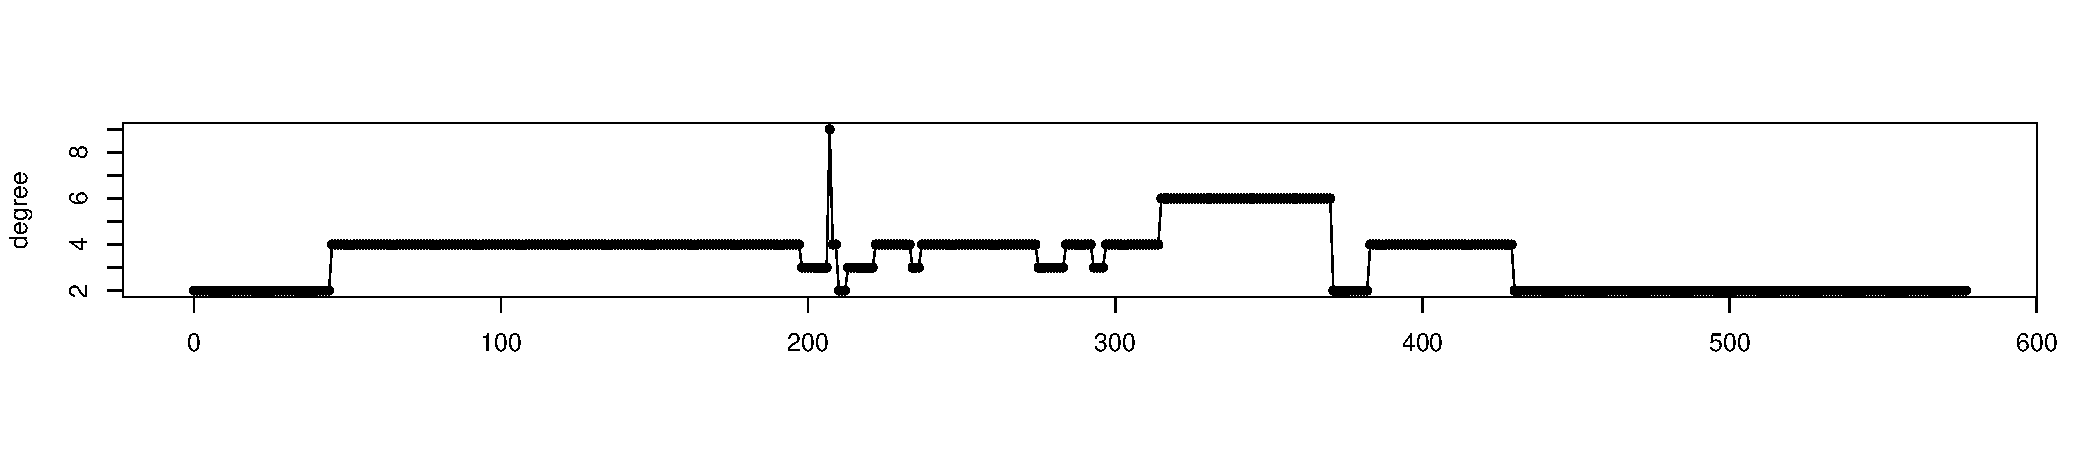
\includegraphics[width=\linewidth,trim=+.225cm 0 +.425cm +2cm]{fig/metrics/chr4_HTT_chm13_degree_w1_bed.pdf}  
  \includegraphics[width=\linewidth]{fig/odgi_tools.pdf}
  \caption{Methods provided by ODGI (in black) and their supported input and output data formats (in brown).}
  \label{fig:operations}
\end{figure*}


\section{Overview}

ODGI provides a set of interrogative and manipulative operations on pangenome graphs.
We have established these tools to support our exploration of graphs built from hundreds of large eukaryotic genomes.
ODGI's tools are practical and able to work with high levels of graph complexity, even with regions where paths present very high depth nodes (10$^5$ to 10$^6$-fold depth).
ODGI covers common operations that we have found to be essential when working with complex pangenome graphs:

%\FIXME{Update the references to the sections.}
\begin{itemize}
\item~\textit{odgi build} constructs the ODGI data model from GFA file (\S\ref{sec:build}).
\item~\textit{odgi view} converts the ODGI data model into GFA file (\S\ref{sec:build}).
\item~\textit{odgi viz} provides a linear visualization of the graph (\S\ref{sec:viz}).
\item~\textit{odgi draw} renders a 2D image of the graph (\S\ref{sec:viz}).
\item~\textit{odgi extract} excerpts subsets of the graph based on path ranges (\S\ref{sec:supp_edit}).
\item~\textit{odgi explode} breaks the graph into connected components (\S\ref{sec:supp_edit}).
\item~\textit{odgi squeeze} unifies disjoint graphs (\S\ref{sec:supp_edit}).
\item~\textit{odgi chop} breaks long nodes into shorter ones (\S\ref{sec:supp_edit}).
\item~\textit{odgi unchop} combines unitig nodes (\S\ref{sec:supp_edit}).
\item~\textit{odgi break} removes cycles in the graph (\S\ref{sec:supp_edit}).
\item~\textit{odgi prune} removes complex regions (\S\ref{sec:supp_edit}).
\item~\textit{odgi groom} resolves spurious inverting links (\S\ref{sec:supp_edit}).
\item~\textit{odgi position} lifts coordinates between path and graph positions (\S\ref{sec:untangle}).%
%\item \textit{odgi server} provides a HTTP server to lift coordinates (\S\ref{sec:untangle}).
\item~\textit{odgi untangle} deconvolutes paths relative to a reference (\S\ref{sec:untangle}).
\item~\textit{odgi tips} finds path end points relative to a reference (\S\ref{sec:supp_navigation}).
\item~\textit{odgi sort} orders the graph nodes (\S\ref{sec:sort}).
\item~\textit{odgi layout} establishes a 2D layout (\S\ref{sec:sort}).
\item~\textit{odgi matrix} derives the pangenome matrix (\S\ref{sec:supp_metrics}).
\item~\textit{odgi paths} lists and extracts paths in FASTA (\S\ref{sec:supp_metrics}).
\item~\textit{odgi flatten} converts the graph to FASTA and BED (\S\ref{sec:supp_metrics}).
\REVIEWED{\item~\textit{odgi pav} computes presence-abscence variations (\S\ref{sec:supp_metrics}).}
\item~\textit{odgi stats} provides numerical properties of the graph (\S\ref{sec:metrics}).
\item~\textit{odgi bin} generates a summarized view of the graph (\S\ref{sec:supp_metrics}).
\item~\textit{odgi depth} describes node depth over graph and path positions (\S\ref{sec:metrics}).
\item~\textit{odgi degree} describes node degree over graph and path positions (\S\ref{sec:metrics}).
\end{itemize}

Each tool focuses on a small set of related operations.
Most read or write the native ODGI format (`og' extension) (Figure~\ref{fig:operations}) and work with standard text based data formats common to bioinformatics.
This supports the implementation of flexible and composable graph processing pipelines based on graphs (GFA/ODGI) and standard bioinformatic data types representing positions, genomic ranges (BED), and pairwise mappings (PAF).
%While the pangenome graph is a first-class entity in ODGI,
% develop a universal, stable, coordinate system, rendering these data types relative to reference and query sequences embedded in the graph.
%To develop a stable and compatible coordinate system,
We use variation graph paths to provide a universal coordinate system, representing annotations and pairwise sequence relationships using the paths as reference and query sequences.
%This avoids the complexity of establishing a stable coordinate system over the topology of the graph, which may change when it is modified or subset.
%Although they present new complexities, we find that pangenome graphs are compatible with current standard ways of working with bioinformatics data.
Thus, ODGI provides a set of interfaces that let us approach these graphs from the perspective of standard reference- and sequence-based data models.
Indeed, by considering all paths in the graph as potential reference or query sequence, we make graphs invisible to downstream tools that operate on collections of sequences or rely on a reference sequence (\textit{e.g.} SAMtools~\citep{Li2009}), enabling interoperability.
This approach benefits from the information in the graph without \REVIEWED{requiring that we build an entirely new set of bioinformatic methods to work} in this difficult new \REVIEWED{pangenomic} research context.

%We begin with a set of HandleGraph-based algorithms first establish in the VG toolkit \citep{Garrison:2018}.
%These include algorithms for graph traversal, partition-finding, $k$-mer and character enumeration, sorting, and pruning.
%Unlike VG, we provide no methods to construct graphs, map reads to the graph, or derive variants.

%Most of the tools are designed to be applied together, piping the output of one tool into the next, thereby preventing the creation of intermediate files, and reducing the number of IO operations.


\subsection{Building the \textsc{ODGI} model}
\label{sec:build}
ODGI maintains its own efficient binary format for storing graphs on disk.
We begin by transforming the storage model of the standard GFAv1~\citep{GFA} format (in which nodes, edges, and paths are described independently) into the ODGI node-centric encoding with \textit{odgi build}.
This construction step can be a significant bottleneck, in particular as the size of the path set of the graph increases. \REVIEWED{The process itself is lossless. A graph in ODGI format represents everything that is in the input GFAv1 graph, without any loss of information.} \REVIEWED{ODGI does not natively support GFAv2 or rGFA.
GFAv2 is similar to GFAv1, but includes process-related annotations of assembly graphs not relevant for pangenome analyses.
rGFA embeds a single coordinate hierarchy over the graph that links all sequences into a single base reference genome.
This positional model depends on a particular graph induction algorithm~\cite{Li:2020}.
In contrast, ODGI implements coordinate translation dynamically (e.g. \textit{odgi position} and \textit{odgi untangle}), allowing use of any embedded genome as a reference.
Its input graphs can represent any kind of alignment between the genomes.
GFAv1 is fully capable of representing many reference genome coordinate systems simultaneously, which supports a reference-agnostic approach that uses the entire pangenome sequence space as a reference system.
In doing so, our approach has the advantage of maintaining backward compatibility with existing tools based on genome sequences.
%ODGI's methods help us to use the pangenome graph model as a coordinating system for analyses that span the entire sequence space of the pangenome.
}

The ODGI data structure (Algorithm~\ref{alg:structs}) allows algorithms that build and modify the graph to operate in parallel, without any global locks.
In \textit{odgi build}, we initially construct the node vector in a serial operation that scans across the input GFA file.
Then, we serially add edges in the $Node.edges$ vectors of pairs of nodes.
Finally, we create paths in serial, and extend them in parallel by obtaining the mutex $Node.lock$ for pairs of nodes and by adding the path step in their $Node.path\_steps$ vectors.
This parallelism speeds ODGI model construction by many-fold when testing against graphs made from assemblies produced by the HPRC (\S\ref{sec:evaluation}).

To support interchange with other pangenome tools or text-based processing, \textit{odgi view} converts a graph in ODGI binary format to GFAv1.
\REVIEWED{ODGI utilizes the PanSN~\citep{pansn-spec} specification to embed sample and haplotype information in the sequence name.
This harmonizes the biosample information present in FASTA, GFA, PAF, VCF, BED, BEDPE, SAM/BAM, and GFF/GTF formats related to the graph and its embedded genome sequences.
%Although this convention may surprise
%we believe that there is vastly greater value to harmonizing our work with existing systems than 
By embedding all sequences into a single hierarchical namespace related to fundamental biological groupings in the input (e.g. biosample, individual, pooled group), PanSN allows us to utilize all assemblies in the pangenome as a combined reference coordinate model.
%This pattern is directly backward\cite{Garrison:2018}.
%Just as rGFA introduces a coordinate hierarchy, PanSN applies a naming hierarchy to all sequences in the pangenome.
%Although many This simple practice is sufficient for all lossless variation graph models.
}
%ODGI uses the ``S'' and ``L'' records to describe the graph topology, and ``P'' records to describe paths.

\section{Results}

\REVIEWED{%Understanding pangenome graphs is not trivial.
Here, we apply our methods to a series of analyses, highlighting how ODGI can assist in exploring the biological features of pangenome graphs.
We follow typical analyses that we have found critical to interpreting whole genome alignments represented in the variation graph model.}

\REVIEWED{To simplify our exposition, we will extract small graph regions that are easy to interpret and describe.
We focus on a handful of difficult loci from the human pangenome, extracting them from a prototype human pangenome graph built with the Pangenome Graph Builder pipeline~\citep{pggb}.
Pangenome graphs built from hundreds of haplotype-resolved \textit{de novo} genome assemblies are very large, but it is often only necessary to work with only a small portion of the genomes represented,
such as a specific locus (Fig.~\ref{fig:viz_extract_untangle-MHC}) or a smaller region (Fig.~\labelcref{fig:viz_extract_untangle-C4-default,fig:viz_extract_untangle-C4-gradient,fig:viz_extract_untangle-C4-strandness,fig:viz_extract_untangle-C4-coverage,fig:viz_extract_untangle-C4-bandage,fig:viz_extract_untangle-C4-bandage-zoom}), or even a single gene (Fig.~\ref{fig:metrics}).
This simplifies the downstream analyses and reduces the resources to work only with the extracted graphs. More on graph extraction and edit operations can be found at $\S$\ref{sec:supp_edit}.}
%Subsetting operations allow us to zoom in on particular genes or regions of interest for more precise examination.

\subsection{Visualizing pangenome graphs}
\label{sec:viz}

% interesting that we don't go base-level at all... we use vg for that, or STM

\REVIEWED{Visualization methods help us quickly gain insight into otherwise opaque biological data.
We find visualization essential for understanding pangenome graphs.}
We pursue a novel approach to visualization with \textit{odgi draw} and \textit{odgi viz}, two tools that provide scalable ways of generating \REVIEWED{raster images showing} the high-level structure of even large pangenome graphs (Fig.~\ref{fig:odgi_viz}).

\REVIEWED{Using \textit{odgi extract}, we extracted the major histocompatibility complex (MHC) locus from a 90-haplotype human chromosome 6 pangenome graph from the HPRC.
Specifically, the graph contains the human references GRCh38, CHM13, and the contigs of 44 diploid individuals that encode all possible variations including those in telomeres and centromeres.
The MHC genes are involved in antigen presentation, inflammation regulation, the complement system, and the innate and adaptive immune responses~\citep{Shiina2009}.
MHC genes are highly polymorphic, i.e., there are multiple different alleles across individuals in a population.
Such variability becomes evident when we apply \textit{odgi draw} to visualize the graph layout of a human MHC pangenome graph (Fig.~\ref{fig:viz_extract_untangle-MHC}) (of note, \textit{odgi layout} first generates the drawn projection, see \S\ref{sec:sort}).
The visualization displays the graph topology in 2 dimensions (2D), with structural variation that appears as bubbles in the layout.}
A 2D rendering can be costly to compute, but we provide an implementation that scales linearly with pangenome sequence size, allowing us to apply it to large pangenome graphs.
%\REVIEWED{For example, \textit{odgi draw} took 6 minutes and 21 seconds in total to produce the 2D layout of the MHC locus (Fig.~\ref{fig:odgi_layout}).}

\REVIEWED{The MHC locus includes the complement component 4 (C4) region, which encodes proteins involved in the complement system.
In Fig.~\ref{fig:viz_extract_untangle-MHC}, C4 corresponds to the small bubble highlighted by the red rectangle.
As an example use case, we took a closer look at the C4 region of the MHC by extracting it from the full MHC pangenome graph with \textit{odgi extract}.
Then, we visualized this subgraph by applying} \textit{odgi viz}, which produces binned, linearized renderings in 1 dimension (1D)\REVIEWED{, where the graph is ordered in 1D across the horizontal axis, with each path represented by a row of the vertical axis} (Fig.~\labelcref{fig:viz_extract_untangle-C4-default,fig:viz_extract_untangle-C4-gradient,fig:viz_extract_untangle-C4-strandness,fig:viz_extract_untangle-C4-coverage}).
For each path, graph nodes are arranged from left to right, with the colored bars indicating the paths and the nodes they cross.
White spaces indicate where paths do not traverse the nodes.
\REVIEWED{Directly consecutive nodes are displayed with no white space between the two.}
The meaning of the colors depends on how \textit{odgi viz} is executed.
By default, path colors are derived from the path names (Fig.~\ref{fig:viz_extract_untangle-C4-default}), which are displayed on the left of the paths.
The black lines on the bottom indicate the edges connecting the nodes and, therefore, represent the graph topology (see \S\ref{sec:supp_visualization} for a more detailed explanation).
This visualization is computed in linear-time and offers a human-interpretable format suitable for understanding the topology and genome relationships in the pangenome graph.
\REVIEWED{In humans, the C4 gene exists as 2 functionally distinct genes, \textit{C4A} and \textit{C4B}, which both vary in structure and copy number~\citep{Sekar_2016}.
In combination with the observed changes in path self-coverage, which represents copy number of a given path relative to the graph (Fig.~\labelcref{fig:viz_extract_untangle-C4-coverage}), the longer link at the bottom of Fig.~\labelcref{fig:viz_extract_untangle-C4-default,fig:viz_extract_untangle-C4-gradient,fig:viz_extract_untangle-C4-strandness,fig:viz_extract_untangle-C4-coverage} indicates that the copy number status of these genes varies across the haplotypes represented in the pangenome.
Moreover, the short nested variation on the left of the locus highlights that \textit{C4A} and \textit{C4B} genes segregate in both long and short genomic forms, distinguished by the presence or absence of a human endogenous retroviral (HERV) sequence.}

Nevertheless, complex, nonlinear graph structures are difficult to interpret in a low number of dimensions.
To overcome this limitation, \textit{odgi viz} supports multiple visualization modalities (Fig.~\labelcref{fig:viz_extract_untangle-C4-gradient,fig:viz_extract_untangle-C4-strandness,fig:viz_extract_untangle-C4-coverage}), making it easy to grasp the properties and shape of the graph.
%Graph node order can affect downstream analyses on pangenome graphs.
For example, we can color the paths by path position (Fig.~\ref{fig:viz_extract_untangle-C4-gradient}), with light grey indicating where paths begin and dark grey where they end.
This visualization is suitable for understanding graph node order, as smooth color gradients indicate that the node order respects the linear paths' coordinate systems.
Pangenome graphs can represent both strands \REVIEWED{of the genomic sequences of the DNA}.
We can display such information by coloring the paths by orientation, with paths colored where their sequence is reverse-complemented (red) or in direct orientation (black) with respect to the sequences of the graph nodes (Fig.~\ref{fig:viz_extract_untangle-C4-strandness}).
%Eukaryotic genomes experience gains and losses of genetic material, resulting in copy number variation (CNV) across the population.
Furthermore, we can use multiple color palettes to color the paths \REVIEWED{by how many times they traverse a node, which can be referred to as the path's depth or coverage of the node, the node depth.}
\REVIEWED{This highlights that in the C4 pangenome graph, the haplotypes present different number of copies of the C4 genes (Fig.~\ref{fig:viz_extract_untangle-C4-coverage}).}

\begin{figure*}[!htb]
    \centering
    \begin{tabular}[t]{c}%{|c|c|}
        %\hline
        \begin{subfigure}[t]{1.0\textwidth}
            \centering
            \caption{\label{fig:odgi_layout}}
            
\includegraphics[width=\linewidth, trim=0cm 18cm -20cm 0.5cm]{fig/extract_viz_draw_position_untangle/chr6_pan_fa_a2fb268_4030258_6a1ecc2_smooth_mhc_H1000w120}
        \end{subfigure} \\
        \begin{tabular}{c}% if you add [t], then sub images are pushed down
            %\smallskip
            \begin{subfigure}[t]{0.5\textwidth}
                \centering
                \caption{}
                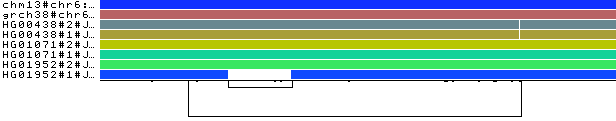
\includegraphics[width=\linewidth, trim=0 1.9cm 0cm 0cm]{fig/extract_viz_draw_position_untangle/chr6_pan_fa_a2fb268_4030258_6a1ecc2_smooth_C4_sorted}
            \end{subfigure} \\
            \begin{subfigure}[t]{0.5\textwidth}
                \centering
                \caption{}
                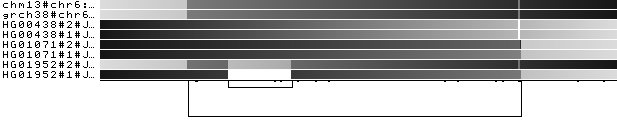
\includegraphics[width=\linewidth, trim=0 +1.9cm 0cm 0cm]{fig/extract_viz_draw_position_untangle/chr6_pan_fa_a2fb268_4030258_6a1ecc2_smooth_C4_sorted_du}
            \end{subfigure} \\
            \begin{subfigure}[t]{0.5\textwidth}
                \centering
                \caption{}
                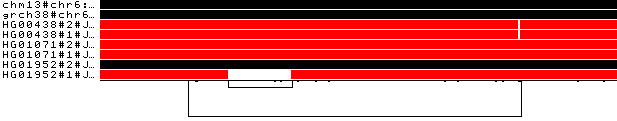
\includegraphics[width=\linewidth, trim=0 +1.9cm 0cm 0cm]{fig/extract_viz_draw_position_untangle/chr6_pan_fa_a2fb268_4030258_6a1ecc2_smooth_C4_sorted_z}
            \end{subfigure} \\
            \begin{subfigure}[t]{0.5\textwidth}
                \centering
                \caption{}
                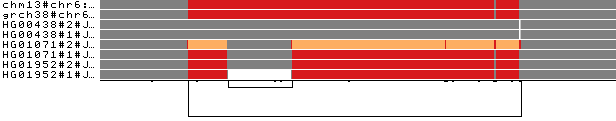
\includegraphics[width=\linewidth, trim=0 +1.9cm 0cm 0cm]{fig/extract_viz_draw_position_untangle/chr6_pan_fa_a2fb268_4030258_6a1ecc2_smooth_C4_sorted_m}
            \end{subfigure}
        \end{tabular}
        %&
        \begin{tabular}{c}% if you add [t], than sub images are pushed down
            %\smallskip
            \\\\
            \begin{subfigure}[t]{0.5\textwidth}
                \centering
                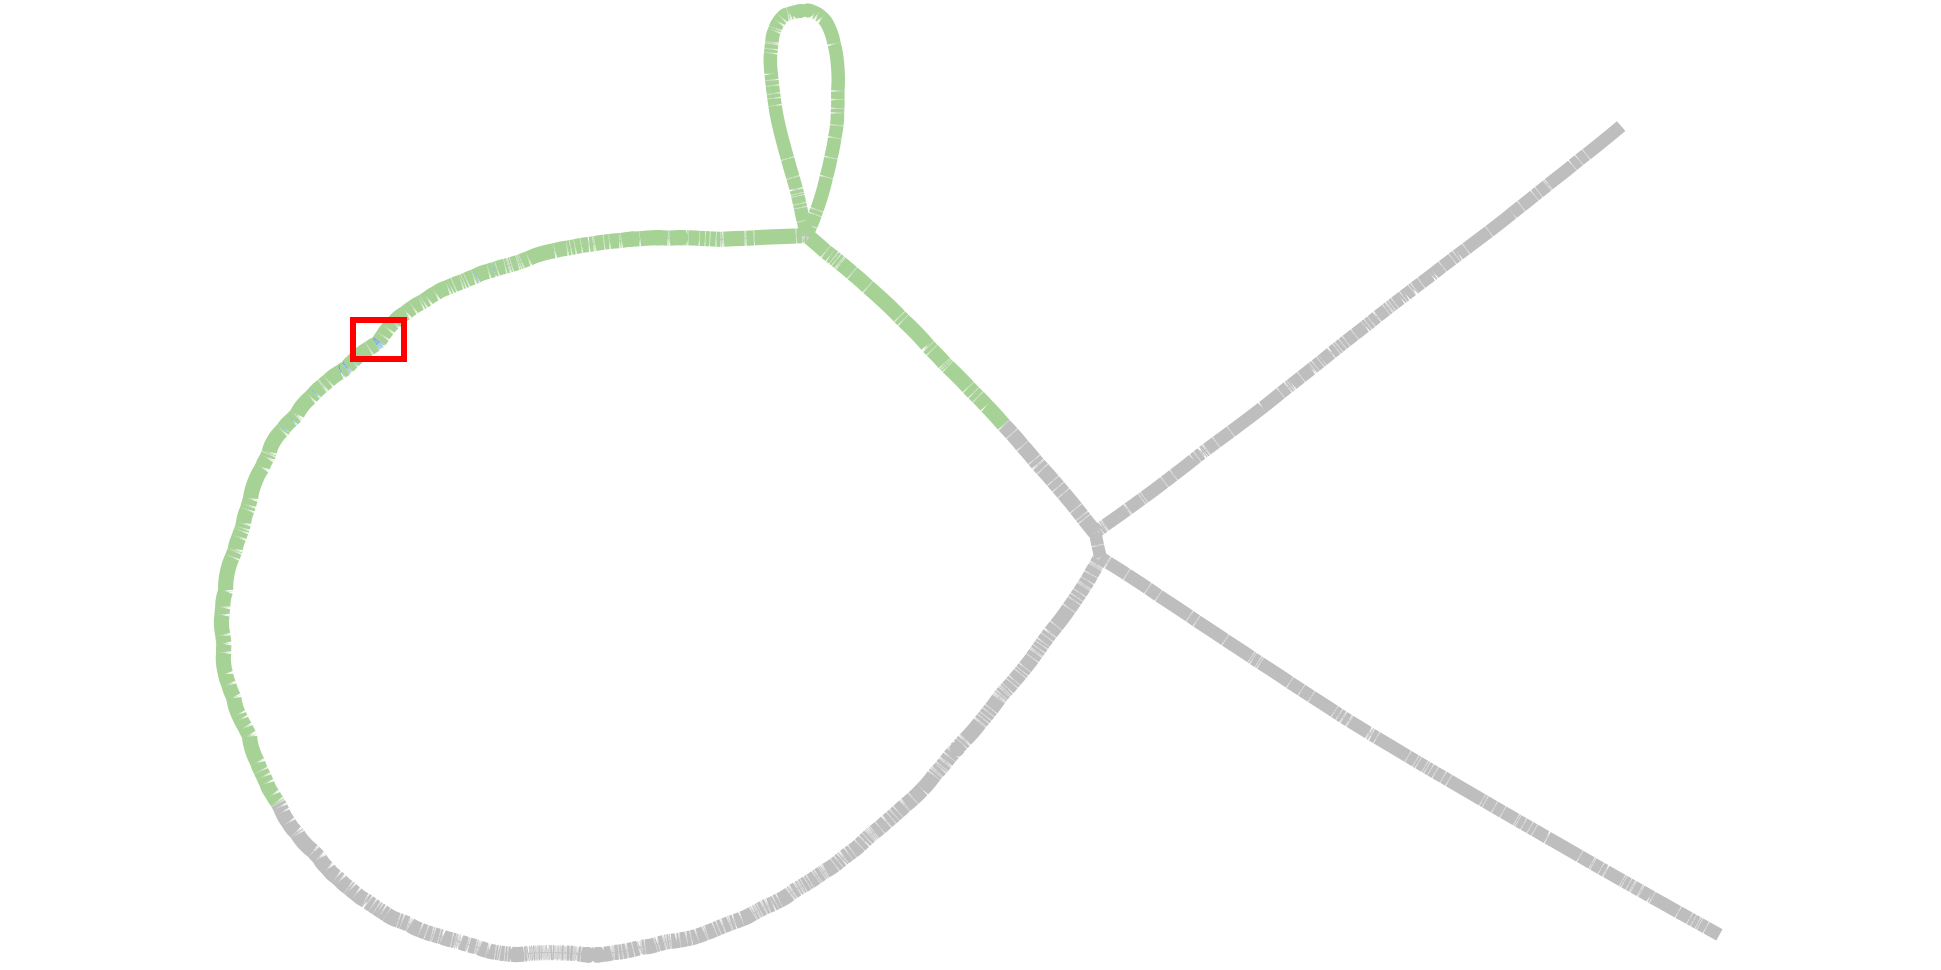
\includegraphics[width=0.65\linewidth, trim=0 +2cm 0 0.5cm]{fig/extract_viz_draw_position_untangle/chr6_pan_fa_a2fb268_4030258_d9f1245_smooth_gfa_C4_sorted_bandage}
                \caption{}
            \end{subfigure}
            \\\\
            \begin{subfigure}[t]{0.5\textwidth}
                \centering
                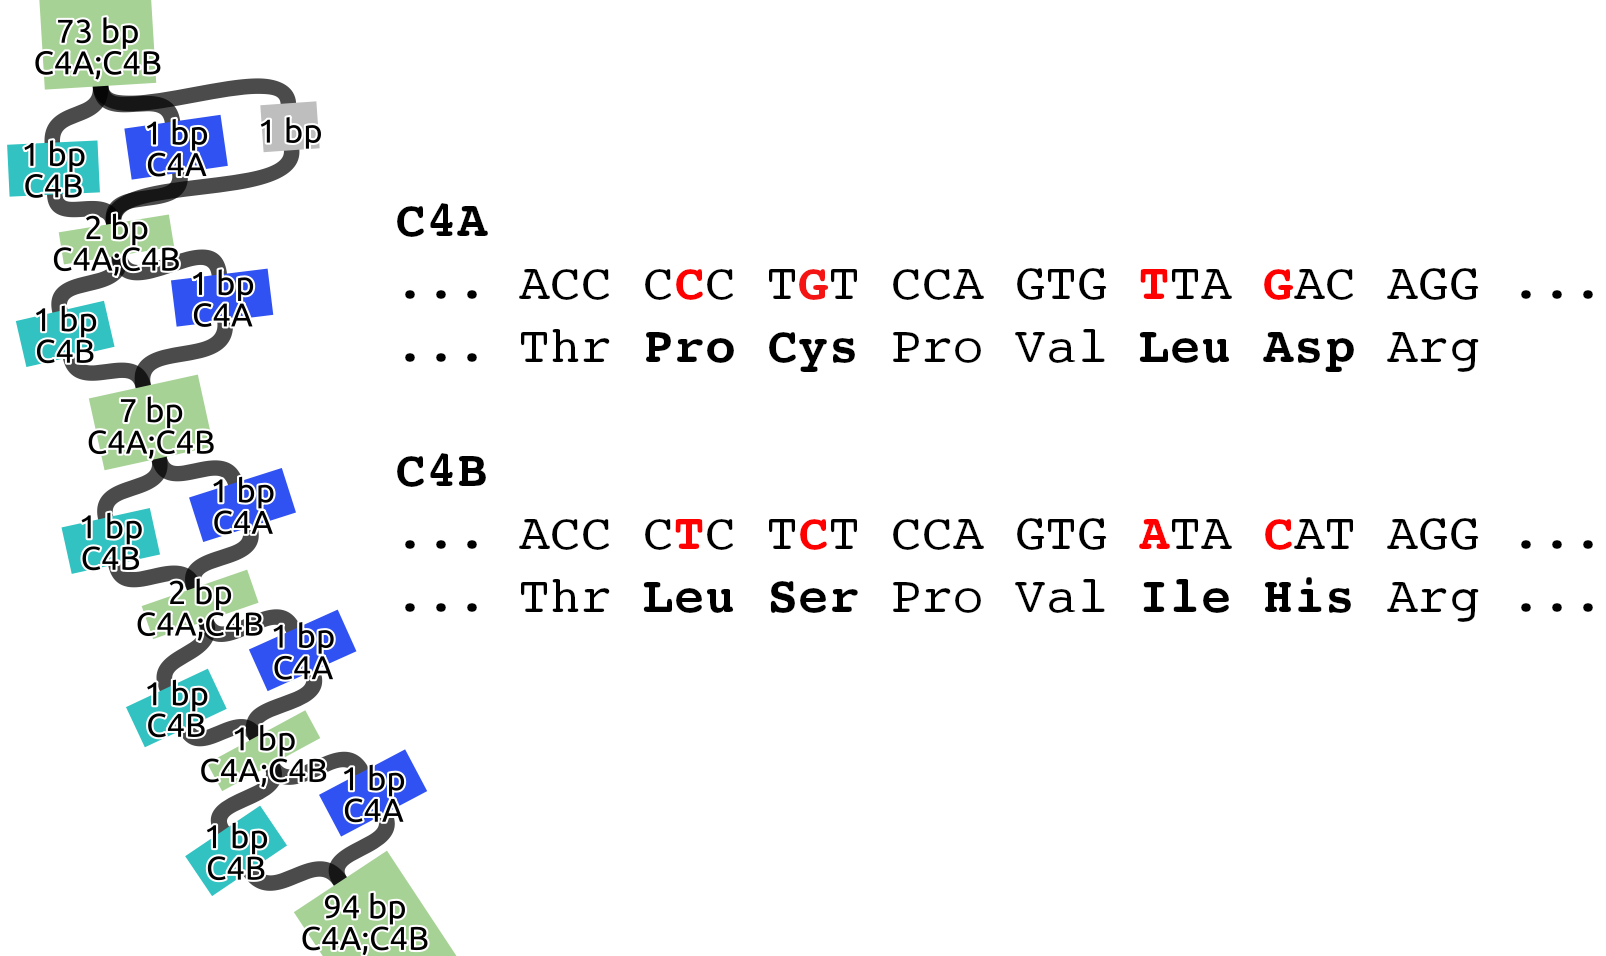
\includegraphics[width=0.65\linewidth, trim=0 +8cm 0 0.5cm]{fig/extract_viz_draw_position_untangle/chr6_pan_fa_a2fb268_4030258_d9f1245_smooth_gfa_C4_sorted_bandage_zoom_in}
                \caption{}
            \end{subfigure}
        \end{tabular}\\
        \begin{subfigure}[t]{1.0\textwidth}
            \centering
            \caption{}
            \begin{center}
                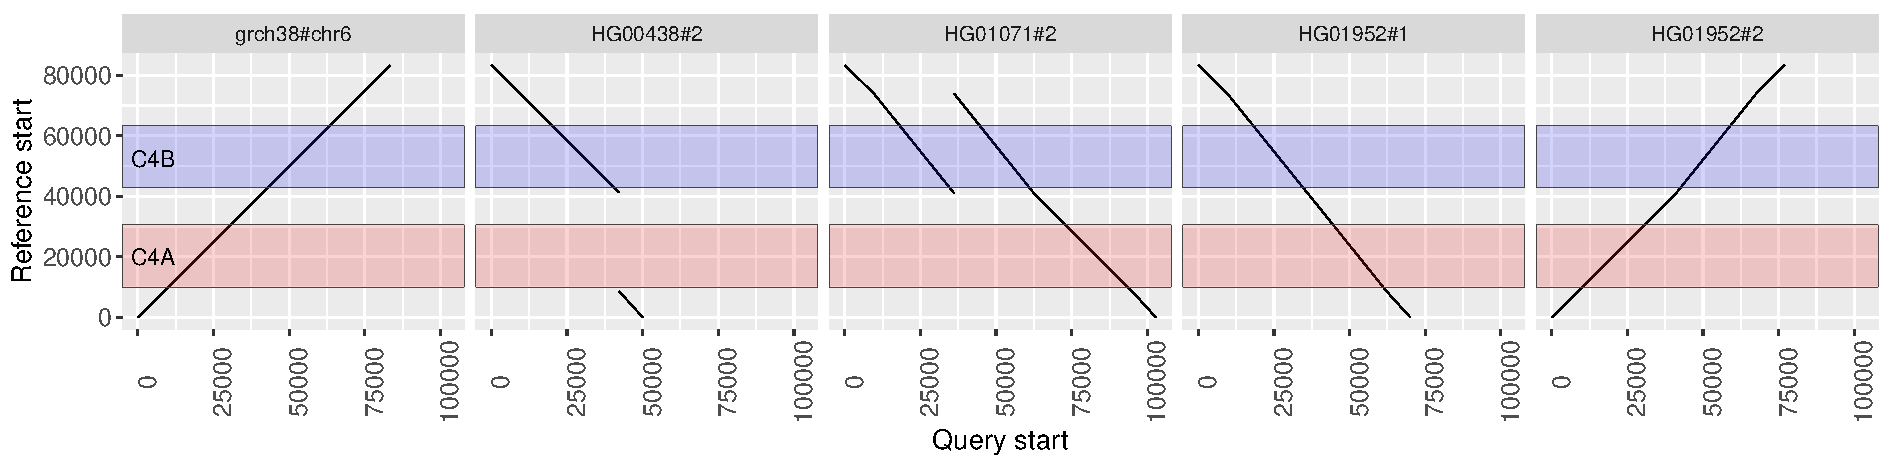
\includegraphics[width=\linewidth, trim=0cm 0.9cm -2.5cm 0.5cm]{fig/extract_viz_draw_position_untangle/chr6_pan_fa_a2fb268_4030258_6a1ecc2_smooth_C4_sorted_untangle_bed}
            \end{center}
        \end{subfigure} \\
        %\hline
    \end{tabular}
    \caption{
        Visualizing the \REVIEWED{major histocompatibility complex (MHC) and complement component 4 (C4)} pangenome graphs. \textbf{(a)} \textit{odgi draw} layout of the MHC pangenome graph extracted from a whole human pangenome graph of 90 haplotypes.
        \REVIEWED{The MHC locus is located on the human chromosome 6 and it encodes molecules involved in antigen presentation, inflammation regulation, the complement system, and the innate and adaptive immune responses~\citep{Shiina2009}.}
        The red rectangle highlights the C4 region\REVIEWED{, which encodes proteins involved in the complement system.}
        \textbf{(b-e)} \textit{odgi viz} visualizations of the C4 pangenome graph, where 8 paths are displayed: 2 reference genomes (chm13 and grch38 on the top) and 6 haplotypes of 3 individuals.
        \textbf{(b)} \textit{odgi viz} default modality: the image shows a quite linear graph.
        The longer links at the bottom indicate the presence of a structural variant (long link) with another structural variant nested inside it (short link on the left).
        Indeed, human C4 exists as 2 functionally distinct genes, \textit{C4A} and \textit{C4B}, which both vary in structure and copy number~\citep{Sekar_2016}. The longer link indicates that the copy number status varies across the haplotypes represented in the pangenome.
        Moreover, \textit{C4A} and \textit{C4B} genes segregate in both long and short genomic forms, distinguished by the presence or absence of a human endogenous retroviral (HERV) sequence, as also highlighted by the short nested link on the left.
        \textbf{(c)} Color by path position. %: the color gradients are smooth, highlighting that its node are well sorted in 1 dimension.
        The top two reference genomes and 2 haplotypes (HG01952\#2) go from left to right, while 5 haplotypes go in the opposite direction, as indicated by the black color on their left.
        \textbf{(d)} \textit{odgi viz} color by strandness: the red paths indicate the haplotypes that were assembled in reverse with respect to the 2 reference genomes.
        \textbf{(e)} \textit{odgi viz} color by node depth: using the Spectra color palette with 4 levels of node depths, white indicates no depth, while grey, red, and yellow indicate depth 1, 2, and greater than or equal to 3, respectively.
        Coloring by node depth, we can see that the two references present two different allele copies of the C4 genes, both of them including the HERV sequence.
        The entirely grey paths have one copy of these genes.
        HG01071\#2 presents 3 copies of the \textit{locus} (orange), of which one contains the HERV sequence (gray in the middle of the orange).
        In HG01952\#1, the HERV sequence is absent.
        \textbf{(f)} \REVIEWED{Layout of the C4 pangenome graph made with the \textit{Bandage} tool~\citep{Wick_2015} and} annotated by using \textit{odgi position}. Green nodes indicate the C4 genes. The red rectangle highlights the regions where \textit{C4A} and \textit{C4B} genes differ.
        \textbf{(g)} Annotated \textit{Bandage} layout of the C4 region where \textit{C4A} and \textit{C4B} genes differ due to single nucleotide variants leading to changes in the encoded protein sequences. Node labels were annoted by using \textit{odgi position}.
        \textbf{(h)} Visualization of \textit{odgi untangle} output in the C4 pangenome graph: the plots show the copy number status of the sequences in the C4 region with respect to the grch38 reference sequence, making clear, for example, that in HG00438\#2, the \textit{C4A} gene is missing. \vspace{-1em}
    }
    \label{fig:odgi_viz}
\end{figure*}


%\begin{figure*}[h!]
%    \begin{subfigure}[t]{.50\linewidth}
%        \caption{}
%        \centering
%        % include first image
%        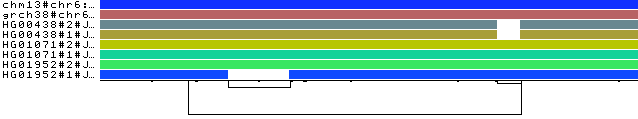
\includegraphics[width=\linewidth, trim=0 +1.5cm -0.5cm 0.5cm]{fig/extract_viz_draw_position_untangle/chr6_pan_fa_a2fb268_4030258_d9f1245_smooth_gfa_C4_sorted}
%        \label{fig:odgi_viz_default}
%    \end{subfigure}
%
%    \begin{subfigure}[t]{.50\linewidth}
%        \caption{}
%        \centering
%        % include second image
%        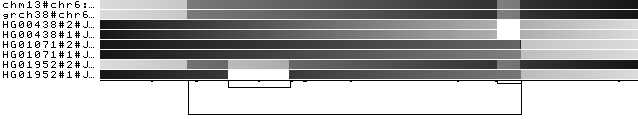
\includegraphics[width=\linewidth, trim=0 +1.5cm -0.5cm 0.5cm]{fig/extract_viz_draw_position_untangle/chr6_pan_fa_a2fb268_4030258_d9f1245_smooth_gfa_C4_sorted_du}
%        \label{fig:odgi_viz_color_by_path_pos}
%    \end{subfigure}
%
%    \begin{subfigure}[t]{.50\linewidth}
%        \caption{}
%        \centering
%        % include second image
%        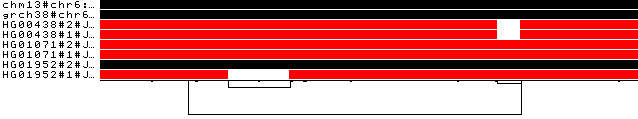
\includegraphics[width=\linewidth, trim=0 +1.5cm -0.5cm 0.5cm]{fig/extract_viz_draw_position_untangle/chr6_pan_fa_a2fb268_4030258_d9f1245_smooth_gfa_C4_sorted_z}
%        \label{fig:odgi_viz_color_by_inversion_rate}
%    \end{subfigure}
%
%    \begin{subfigure}[t]{.50\linewidth}
%        \caption{}
%        \centering
%        % include fourth image
%        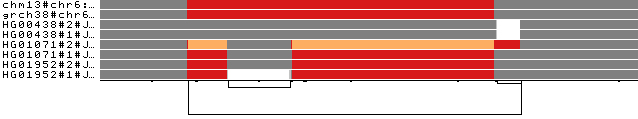
\includegraphics[width=\linewidth, trim=0 +1.5cm -0.5cm 0.5cm]{fig/extract_viz_draw_position_untangle/chr6_pan_fa_a2fb268_4030258_d9f1245_smooth_gfa_C4_sorted_m}
%        \label{fig:odgi_viz_color_by_path_depth}
%    \end{subfigure}
%    \begin{subfigure}[t]{.50\linewidth}
%        \caption{}
%        \centering
%        % include first image
%        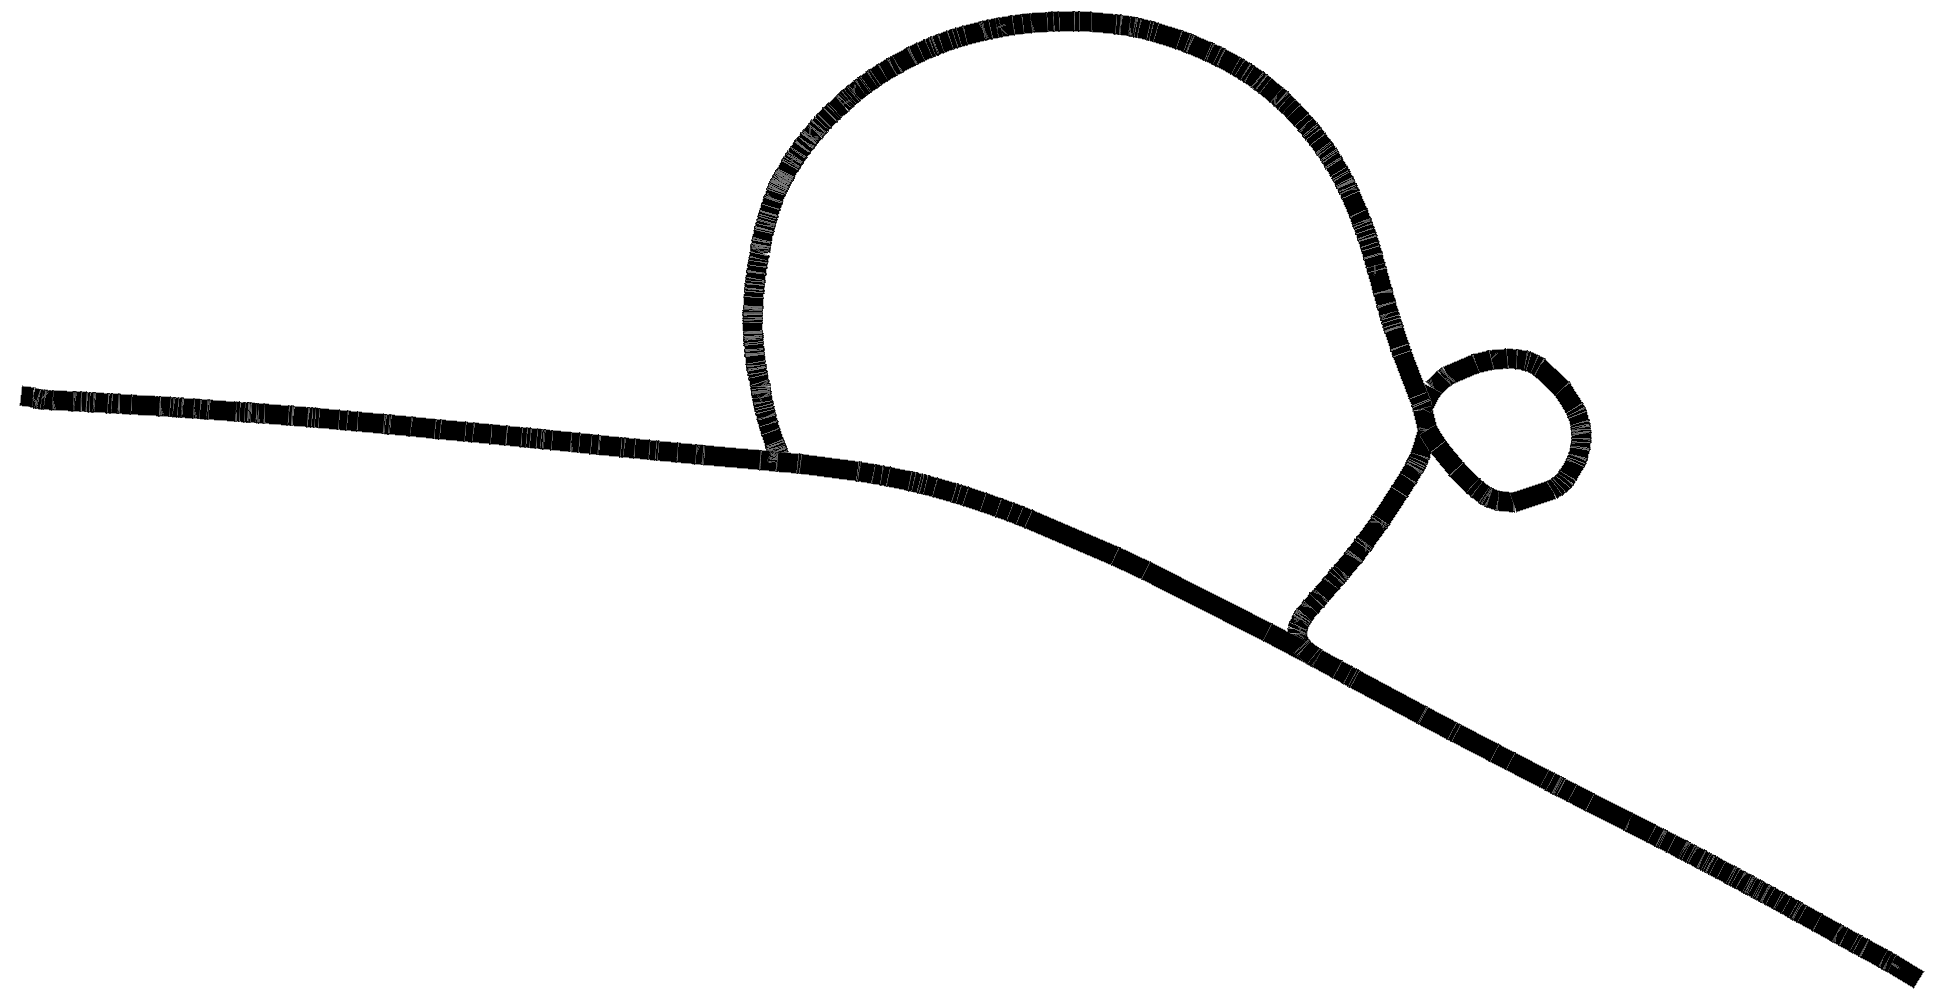
\includegraphics[width=0.5\linewidth, trim=0 +2cm 0 0.5cm]{fig/extract_viz_draw_position_untangle/chr6_pan_fa_a2fb268_4030258_d9f1245_smooth_gfa_C4_sorted_layout}
%        \label{fig:odgi_viz_default2}
%    \end{subfigure}
%    \begin{subfigure}[t]{.50\linewidth}
%        \caption{}
%        \centering
%        % include second image
%        %todo BANDAGE
%        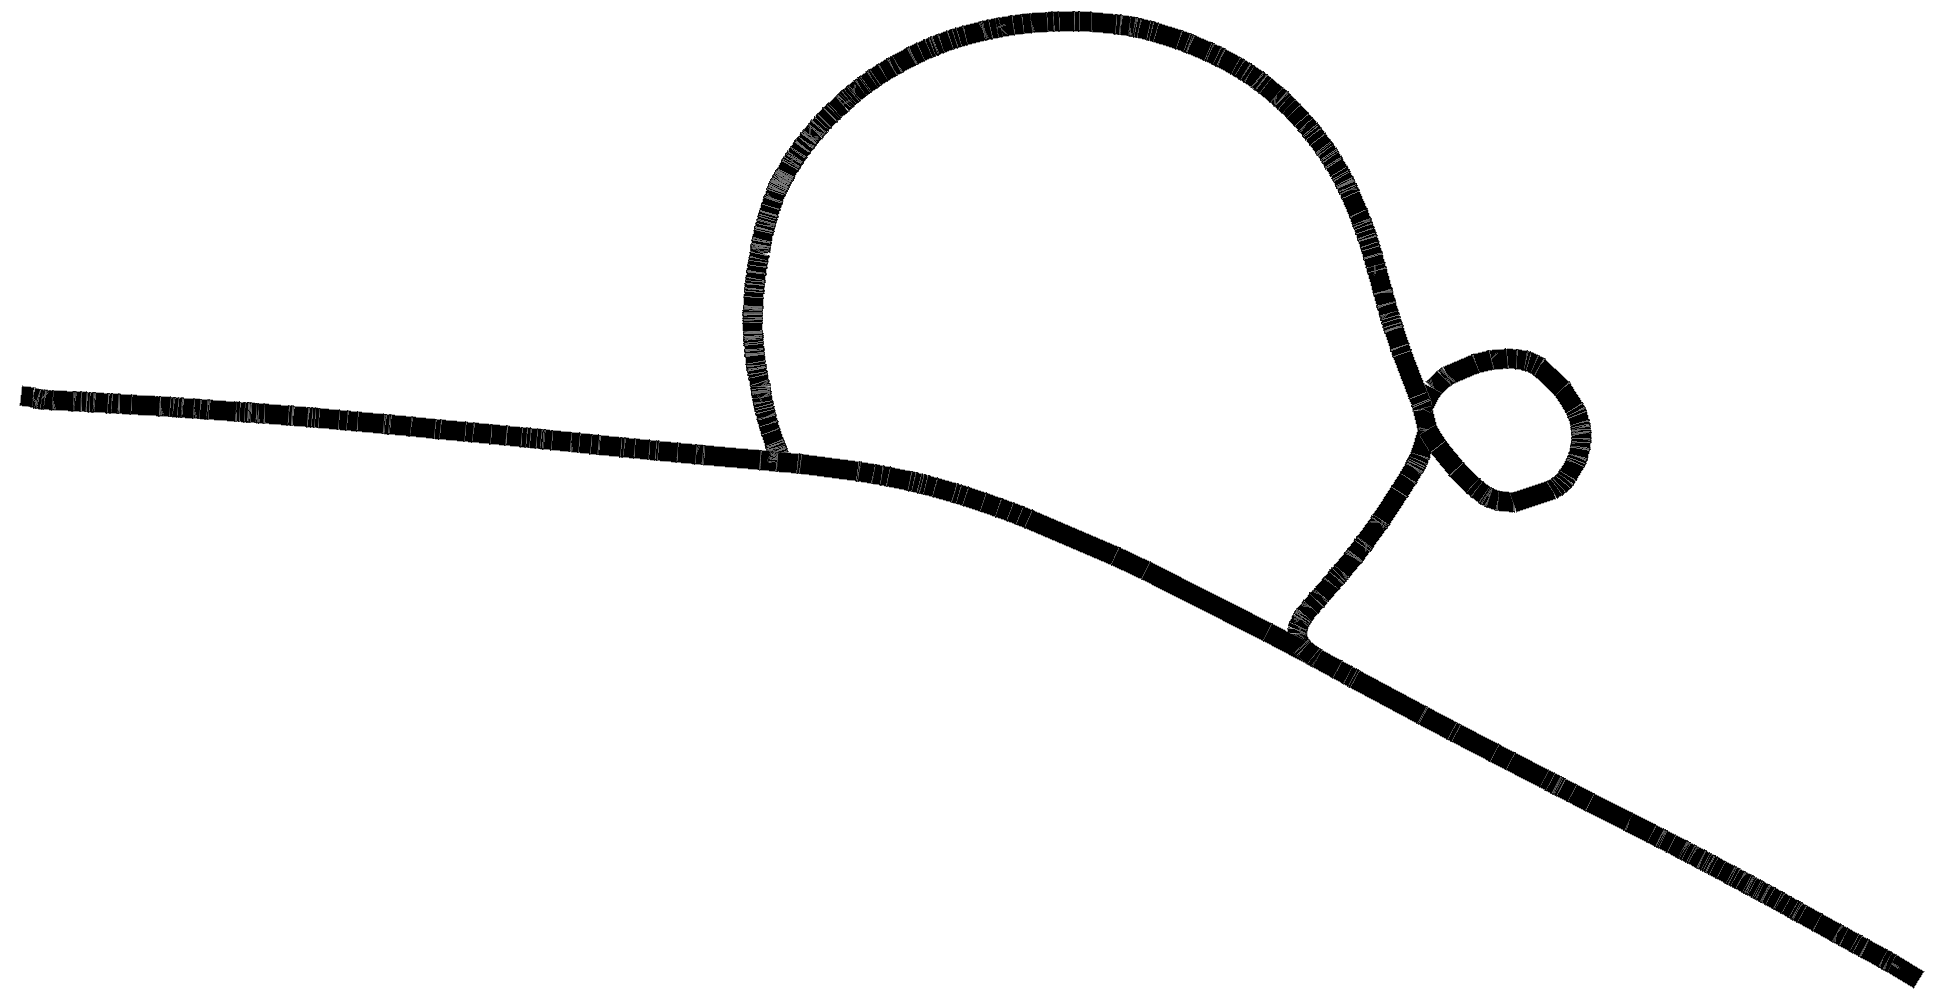
\includegraphics[width=0.5\linewidth, trim=0 +1.5cm -0.5cm 0.5cm]{fig/extract_viz_draw_position_untangle/chr6_pan_fa_a2fb268_4030258_d9f1245_smooth_gfa_C4_sorted_layout}
%        \label{fig:odgi_viz_color_by_inversion_rate2}
%    \end{subfigure}
%
%    \caption{
%        Visualizing the complement component 4 (C4) pangenome graph extracted from a whole human pangenome graph of 90 haplotypes.
%        In all visualizations, 8 paths are displayed: 2 reference genomes (chm13 and grch38 on the top) and 6 haplotypes of 3 individuals.
%        \textbf{(a)} default modality: the image shows a quite linear graph.
%        The longer links at the bottom indicate the presence of a structural variant (long link) with another structural variant nested inside it (short link on the left).
%        Indeed, human C4 exists as 2 functionally distinct genes, C4A and C4B, which both vary in structure and copy number \citep{Sekar_2016}. The longer link indicates that the copy number status varies across the haplotypes represented in the pangenome.
%        Moreover, C4A and C4B genes segregate in both long and short genomic forms, distinguished by the presence or absence of a human endogenous retroviral (HERV) sequence, as also highlighted by the short nested link on the left.
%        \textbf{(b)} color by path position: the color gradients are smooths, highlighting that its node are well sorted in 1 dimension.
%        The top two reference genomes and 2 haplotypes (with name starting with HG01952\#2) go from left to right, while 5 haplotypes go in the opposite direction, as indicated by the black color on their left.
%        \textbf{(c)} color by strandness: the red paths indicate the haplotypes that were assembled in reverse with respect to the 2 reference genomes.
%        \textbf{(d)} color by path depth: using the Spectra color palette with 4 level of path depths, white indicates no depth, while grey, red, and yellow indicate depth 1, 2, and greater than or equal to 3, respectively.
%        Coloring by path depth, we can see that the two references present two different allele copies of the C4 genes, both of them including the HERV sequence.
%        The entirely grey paths have one copy of these genes.
%        The path with name starting with HG01071\#2 presents 3 copies of the genes (indicated by the orange color), of which only 1 with the HERV sequence (gray color in the middle of the orange region).
%        In the haplotype with the name starting with HG01952\#1, the HERV sequence is absent.
%    }
%    \label{fig:odgi_viz}
%\end{figure*}

\subsection{Untangling and navigating the pangenome}
\label{sec:untangle}

%We find that, to understanding relationships between sequences and positions in pangenome graphs, we must use context mapping to ``untangle'' complex regions found in VNTRs, segmental duplications, and centromeric repeats.
%This approach lets use pangenome graphs as a foundation for universal liftover between any two sets of sequences in the graph.

The key data in a pangenome graph is a representation of the alignment (i.e., the homology relationships) between \REVIEWED{genomic sequences}.
Navigating and understanding the graph requires coordinate systems to link other data to the sequences represented in the graph model.
ODGI's tools use the embedded sequences to provide a universal coordinate space that is graph-independent, thereby remaining stable across different graphs built with the same sequences.
Such a a universal coordinate system allows us to support several kinds of ``lift-over'' of coordinates between different sequences in the same or different graphs.
%Our for positional conversion (\textit{odgi position}), annotation liftover (\textit{odgi untangle}), breakpoint identification (\textit{odgi tips}), subgraph extraction (\textit{odgi extract}), visualization (\textit{odgi viz}), path depth (\textit{odgi depth}), and graph complexity measurement (\textit{odgi degree}) can all operate on coordinates of paths in the graph.
\REVIEWED{As a demonstration, we took the C4 pangenome graph and added to its nodes gene annotation from GRCh38 (in GFF format file) using \textit{odgi position} ($\S$\ref{sec:supp_gff}). The resulting TSV contains pairs of nodes and colors. Taking the graph and the TSV into Bandage~\citep{Wick_2015}, the actual C4 genes are highlighted (Fig.~\ref{fig:viz_extract_untangle-C4-bandage}). Zooming to the nucleotide level, the annotation shows the single nucleotide differences of the \textit{C4A} and the \textit{C4B} genes (Fig.~\ref{fig:viz_extract_untangle-C4-bandage-zoom}).}

\textit{odgi position} can also translate graph and path positions between or within graphs, emitting the liftovers in BED format.
For a precise translation process when conversing a query position to a reference position in a repeat region, we apply the \textit{path jaccard} context mapping concept.
It could be that the found reference node is visited several times by the reference.
To ensure a precise translation, we select the reference position whose context (the multiset of $Node.id$s reached within a distance of e.g. 10kbp) has the best jaccard metric when compared to the query context. \REVIEWED{For a more detailed explanation of the \textit{path jaccard} concept see $\S$\ref{sec:supp_path_jaccard}.}
%the best jaccard for the query step and each reference candidate step is calculated by looking at a context range (e.g. 10kbp) around the locus.

% untangle (this follows on the jaccard graph mapping concepts in the previous section}
%We can use coordinates in any genome to refer to it, but this requires a few basic operations ...
%Obtaining unambiguous mappings between different genomes requires the use of a new kind of graph based mapping (path graph jaccard).

\REVIEWED{To obtain a more precise overview of the locus in Fig.~\labelcref{fig:viz_extract_untangle-C4-default,fig:viz_extract_untangle-C4-gradient,fig:viz_extract_untangle-C4-strandness,fig:viz_extract_untangle-C4-coverage},
we applied \textit{odgi untangle} with GRCh38 as a reference.
\textit{odgi untangle} segments paths into linear segments by breaking these segments where the paths loop back on themselves.
In this way, we obtain information on the position and copy number status of the sequences in the collapsed locus, in BEDPE or PAF format.
In the representation in Fig.~\ref{fig:viz_extract_untangle-C4-untangle}, the orientation of the line indicates if the copy number is in forward or in reverse orientation compared to GRCh38.
\textit{odgi untangle} is able to work with any sets of reference sequences, converting the graph to lift-over maps compatible with standard software for projecting annotations and alignments from one genome to another.
An explanation of the untangling process is given in $\S$\ref{sec:supp_navigation}.}
%This lets us decompose both homology and paralogy relationships by also untangling looping motifs in the graph, and obtaining linearized pairs of regions in BEDPE or PAF format.
%As an example, by untangling the graph we can study the variation that lies in regions collapsed due to ambiguous alignments over sequence repeats (as shown in Fig.~\ref{fig:viz_extract_untangle-C4-bandage}).


%Having built a pangenome graph from assembly contigs, we can ask questions like: Where do our contigs' ends match the reference(s)? An answer to this question can highlight regions that are tricky to assemble (Fig. ~\ref{fig:tips}).

\subsection{Latent graph structure reveals underlying biology}
\label{sec:sort}

Pangenome graphs can hide their underlying latent structures, introducing difficulties in the analysis and interpretation. % (Fig.~\ref{fig:sorting}\textbf{a}).
Among the causes of this is the correct ordering of the graph nodes in a convenient number of dimensions.
ODGI provides a variety of sorting algorithms to find the best graph node order in 1 or 2 dimensions, allowing us
to understand the sparse structures typically found in pangenome graphs and the genetic variation they represent.
\REVIEWED{\textit{odgi sort} allows the chaining of these sorting algorithms.
As many of the algorithms are affected by the initial node order, this allows us to generate sorting pipelines that progressively refine the graph ordering.}

\REVIEWED{We applied several of \textit{odgi sort}'s 1D algorithms to a 90-haplotype human MHC pangenome and a C4 subgraph (Fig.~\ref{fig:sorting}).
The randomly sorted MHC graph (Fig.~\ref{fig:mhc-random-node-order}) hides its linear graph structure, whereas our novel path-guided (PG) stochastic gradient descent (SGD) algorithm, PG-SGD, is able to produce a globally linear ordered graph revealing the C4 region (Fig.~\ref{fig:mhc-pgsdg-sorting}).
This exploits path information to order the graph nodes.
%For understanding the large-scale organization of the graph, we benefit from an even simpler coordinate system.
PG-SGD learns a 1D or 2D organization of the graph nodes that matches nucleotide distances in graph paths (i.e., the sequences embedded in the graph).
To scale to large graphs, we learn this projection in parallel via a HOGWILD! approach~\citep{niu2011hogwild}.
PG-SGD can be seen as an adaptation of SGD-based drawing~\citep{zheng2018graph} to pangenome graphs.
In parallel, each HOGWILD! thread updates the relative position of pairs of nodes so that their distance in the layout, or their order, better-matches  their nucleotide distance in the paths running through the graph.
Following standard SGD approaches, the learning rate is reduced as the algorithm progresses, and execution continues until the adjustments to the model fall below a target threshold $\epsilon$.}

\REVIEWED{A PG-SGD sorting of C4 compresses both sides of the variant bubble into one dimension, leading to an interrupted pattern of nodes across the copy-number variable region (Fig.~\ref{fig:c4-pgsdg-sorting}).
Subsequently applying a topological sort clarifies the graph's latent structure, simplifying interpretation (Fig.~\ref{fig:c4-topological-sorting}). }
%
\REVIEWED{To find the best order of graph nodes in 1D, \textit{odgi sort}'s multiple sorting algorithms can be combined into a sorting pipeline to take advantage of the strength of each (results not shown).
ODGI can project vector (in 1D) and matrix (2D) representations of the graph relative to these learned coordinate spaces.
Based on this projection, we can trivially sort graph nodes in 1D.
Moreover, we support the same concept in 2D in \textit{odgi layout} by providing a 2D implementation of the PG-SGD algorithm (Figure~\ref{fig:odgi_layout}). A detailed description of the node ordering process can be found at $\S$\ref{sec:supp_sorting}. As we have shown above, the node order is crucial to understand the biological features of a pangenome graph.}
%As the PG-SGD sorts graph nodes with respect to the paths which walk through them, we can also detect regions whose layout is distorted, which may represent structural variation or assembly error.


\begin{figure}[ht!]
    \begin{subfigure}{\linewidth}
        \caption{}
        \centering
        % include first image
        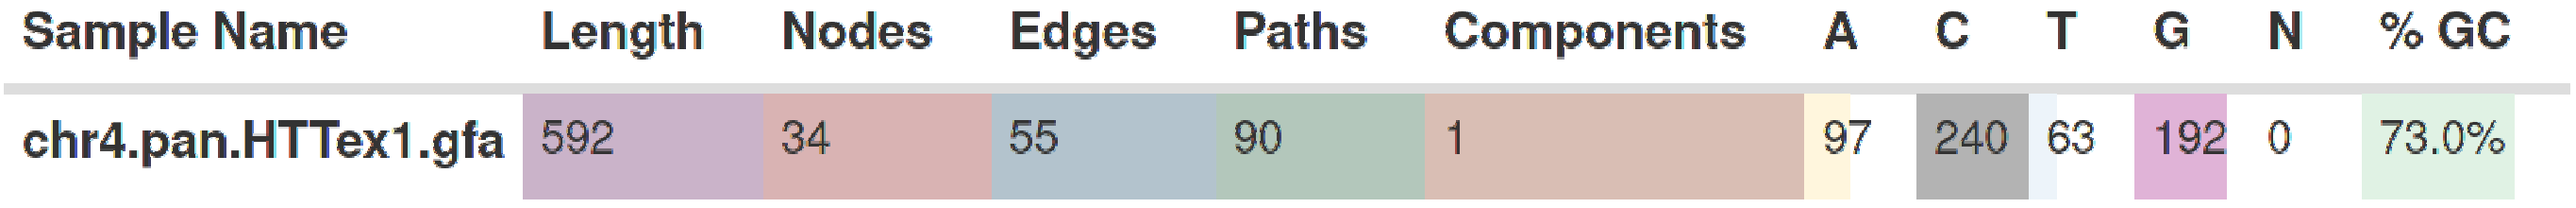
\includegraphics[width=1.0\linewidth, trim=-2.25cm 1.0cm 0cm 3.75cm]{fig/metrics/chr4_pan_HTTex1_gfa_multiqc_odgi_stats_svg}
        \label{fig:metrics-multiqc}
        	\vspace{-2em}
    \end{subfigure}
    \begin{subfigure}{1\linewidth}
        \caption{}
        \centering
        % include fourth image
        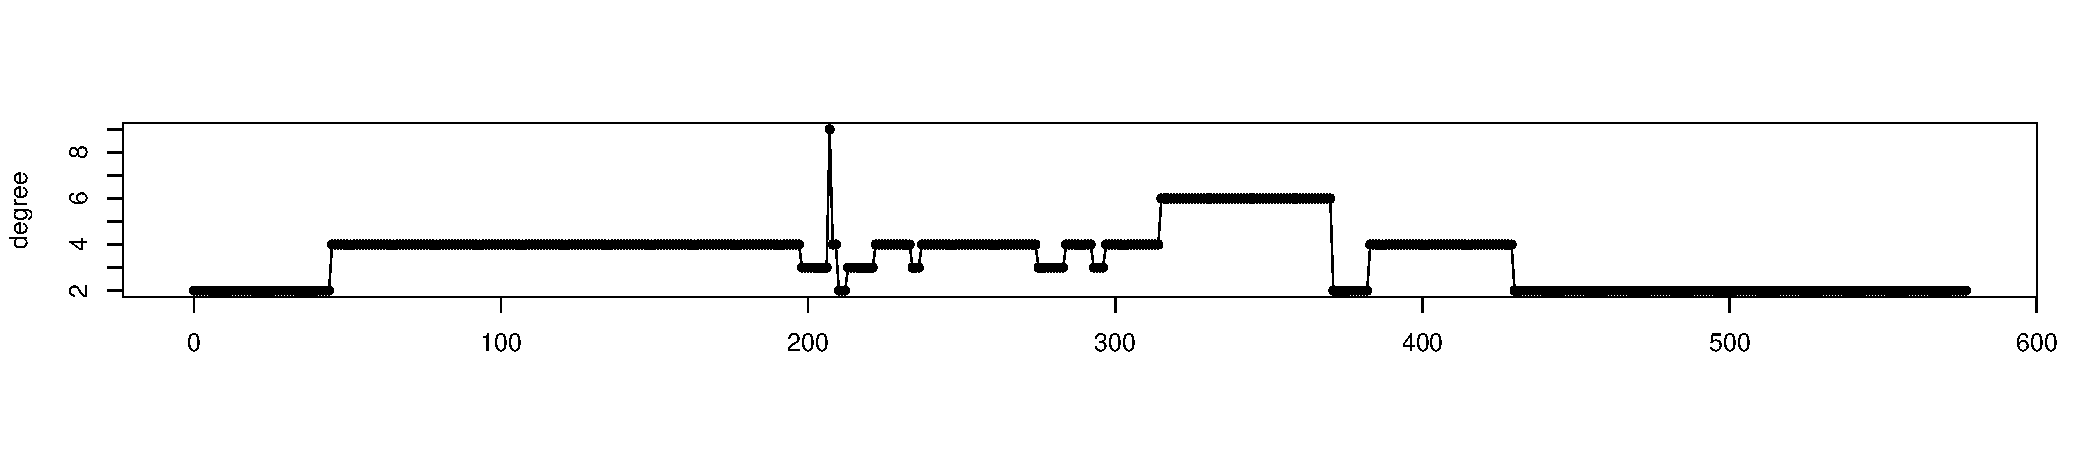
\includegraphics[width=\linewidth,trim=-.225cm 4cm +.425cm +3cm]{fig/metrics/chr4_HTT_chm13_degree_w1_bed}
        \label{fig:metrics-degree}
    \end{subfigure}
    \begin{subfigure}{\linewidth}
        \caption{}
        \centering
        % include second image
        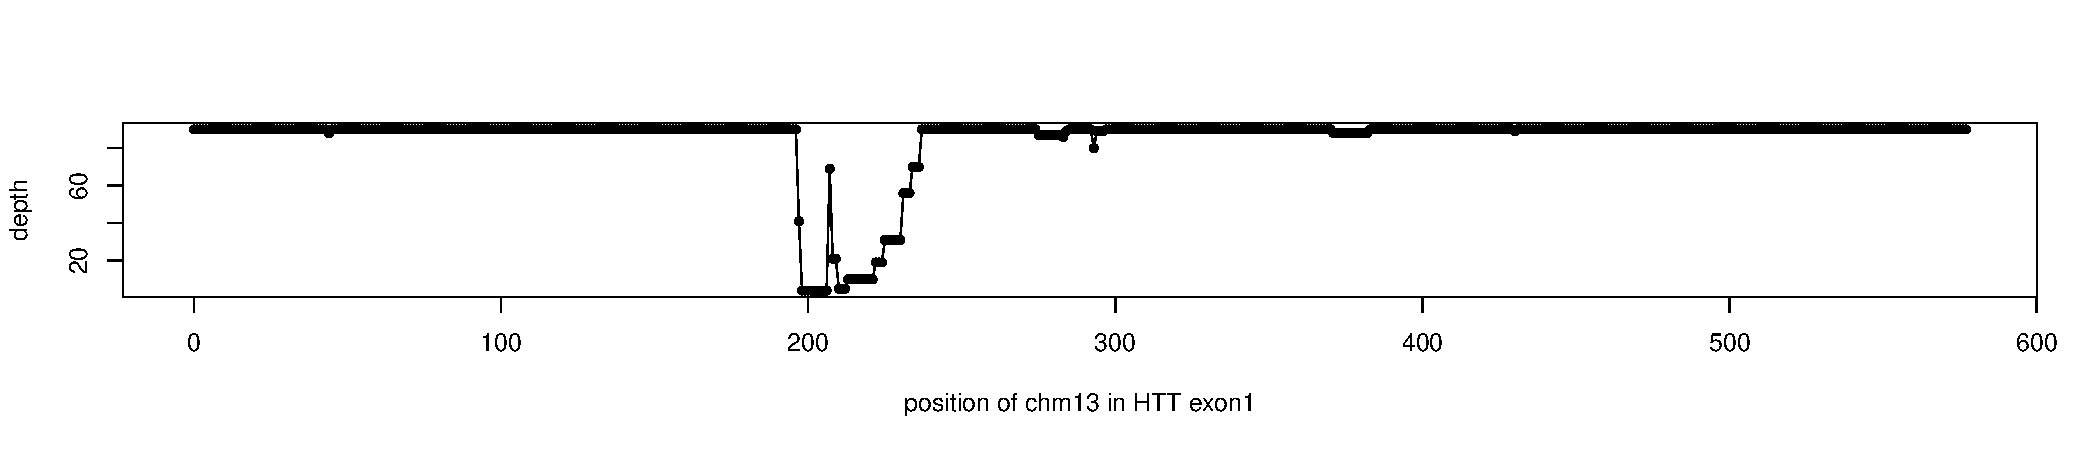
\includegraphics[width=\linewidth,trim=-.225cm 3.3cm +0.425cm +3cm]{fig/metrics/chr4_HTT_chm13_depth_w1_bed}
        \label{fig:metrics-depth}
    \end{subfigure}
    \begin{subfigure}{\linewidth}
        \caption{}
        \centering
        % include second image
        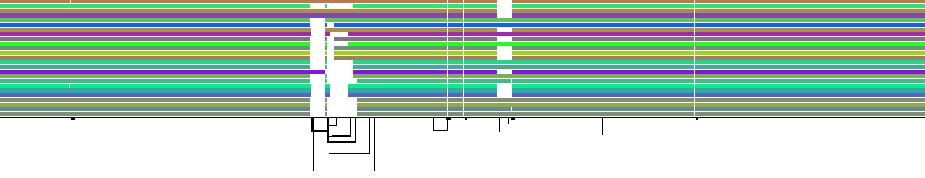
\includegraphics[width=1.0\linewidth, trim=-1.75cm 2.2cm -0.75cm 0.5cm]{fig/metrics/chr4_pan_fa_a2fb268_4030258_6a1ecc2_smooth_gfa_og_HTTex1_og_O_og_tiny_og_png_svg.pdf}
        \label{fig:metrics-viz}
    \end{subfigure}
    \begin{subfigure}{\linewidth}
        \caption{}
        \centering
        % include second image
        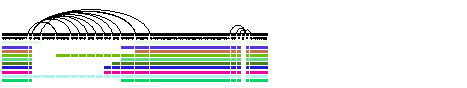
\includegraphics[width=1.0\linewidth, trim=-0.4cm 0.4cm 3.15cm 0cm]{fig/metrics/chr4_pan_HTTex1_STR_xg_svg}
        \label{fig:metrics-str}
        \vspace{-0.5em}
    \end{subfigure}
%	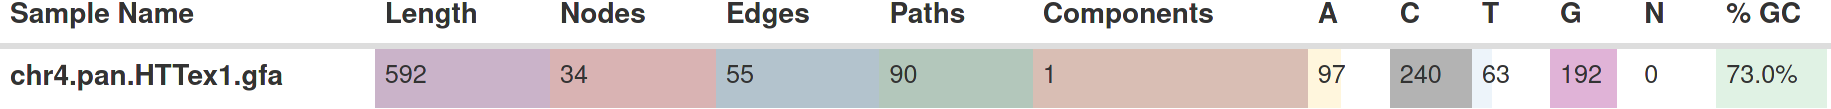
\includegraphics[width=\linewidth]{fig/metrics/chr4.pan.HTTex1.gfa.multiqc_odgi_stats.png}
	\caption{Features of a 90-haplotype human pangenome graph of the exon 1 huntingtin gene (\textit{HTTexon1}): \textbf{(a)} Excerpt of vital statistics of the \textit{HTTexon1} graph displayed by MultiQC's ODGI module. The very high GC content of 73.0\% compared to a human genomic mean GC content of 40.9\% \citep{Piovesan2019} is in accordance with the literature \citep{Neueder2017}. \textbf{(b)} Per nucleotide node degree distribution of CHM13 in the \textit{HTTexon1} graph. Around position 200 there is a huge variation in node degree. \textbf{(c)} Per nucleotide node depth distribution of CHM13 in the \textit{HTTexon1} graph. The alternating depth around position 200 indicates polymorphic variation complementing the above node degree analysis. \textbf{(d)} \textit{odgi viz} visualization of the 23 largest gene alleles, CHM13, and GRCH38 of the \textit{HTTexon1} graph. \textbf{(e)} \textit{vg viz} nucleotide-level visualization of 10 gene alleles, CHM13, GRCH38 of the \textit{HTTexon1} graph focusing on the CAG variable repeat region. Figures \textbf{(b)-(e)} highlight the variant region around position 200 of CHM13 showing the variable number of glutamine residues of the different individuals as reported by \citep{Nance1999}.}
	\label{fig:metrics}
\end{figure}


\subsection{Graph features highlight variation}
\label{sec:metrics}

\REVIEWED{Graphs statistics provide alternative ways to gain insight into pangenomes complexity revealing the overall structure, size, and features of a graph and its sequences.}

\REVIEWED{As a use case study (Fig.~\ref{fig:metrics}), we took a look at the metrics of a 90-haplotype human pangenome graph of the exon 1 huntingtin gene (\textit{HTTexon1}). In particular, we obtained the number of nodes, edges, paths, components, bases, the graph length, and the GC content with \textit{odgi stats}. The output pangenome statistics in YAML textual file format was given to
MultiQC's~\citep{Ewels_2016} newly added ODGI module. As can be seen in Figure~\ref{fig:metrics-multiqc}, we observe a very high GC content of 73.0\% in the \textit{HTTexon1} graph compared to the human genomic mean GC content of 40.9\% \citep{Piovesan2019}. This is in accordance with the literature~\citep{Neueder2017}. %\footnote{\url{https://multiqc.info/docs/\#odgi} (accessed Oct 2021)}
Despite this discovery, the MultiQC module provides an interactive way to comparatively explore statistics of an arbitrary number of graphs.}

\REVIEWED{To investigate in detail which intricate regions in the \textit{HTTexon1} graph are responsible for its genetic variation and high GC content, we took a look at the per nucleotide node degree (Fig.~\ref{fig:metrics-degree}) and node depth (Fig.~\ref{fig:metrics-depth}) distributions of CHM13 by using \textit{odgi depth}'s and \textit{odgi degree}'s BED output, respectively.
The results indicate a highly polymorphic region around position 200 in the graph.
Figure~\ref{fig:metrics-viz} supports this analysis. Zooming in on this region with \textit{vg viz}, we can clearly identify the typical \textit{HTTexon1} CAG variable repeat region (Fig.~\ref{fig:metrics-str}).
Figures~\ref{fig:metrics-degree}-\ref{fig:metrics-viz} highlight the variant region around position 200 of CHM13, showing the variable number of glutamine residues of the different individuals as reported by~\citep{Nance1999}.}
%In general, such complex motives can be the mirror of genetic variation, but also misassemblies or problems in the pangenome building, making the tools further useful for graph validation. Additional graph metrics interrogation tools are detailed in $\S$\ref{sec:supp_metrics}.}

\vspace{0.22cm}

\subsection{Performance evaluation}
\label{sec:evaluation}

\REVIEWED{
Although many of the operations that ODGI provides are unique, some are common with the existing VG toolkit.
We compare with these to highlight the practical performance implications of our graph data structure design.
Our results highlight the efficient parallel algorithm implementations enabled by this design.}

\REVIEWED{We compared the efficiency of ODGI (v0.6.3-56-gebc493f "Pulizia") and VG (v1.37.0 "Monchio") for routine pangenome tasks. In particular, we measured the execution time and memory usage}
\begin{inparaenum}[(i)]
	\item \REVIEWED{of transforming a GFAv1 file into a tool's native format, }
	\item \REVIEWED{the extraction of a subgraph,}
	\item \REVIEWED{the visualization of a pangenome graph, and}
	\item \REVIEWED{the finding of path positions in a pangenome graph.}
\end{inparaenum}
\REVIEWED{These graph operations are key when it comes to the understanding of pangenome graphs.
They are also a set of functions implemented in both toolkits.
We ran these operations for a varying number of threads and haplotypes in the graph for a scaling analysis. We ran each evaluation configuration 10 times and report the mean of each run.
All evaluations were performed on a VM in the German Network for Bioinformatics Infrastructure (deNBI) cloud with 28 cores and 256GB of RAM.
The presented results are from a 90-haplotype chromosome 6 human pangenome graph built with data from the HPRC.
Specifically, the graph contains the human references GRCh38, CHM13, and the contigs of 44 diploid individuals that encode all possible variations including those in telomeres and centromeres.
When transforming a GFAv1 file with VG, the static XG file format was used.
The tools involved in the evaluation process require the XG format.}

\REVIEWED{In general, ODGI makes comparatively better use of multithreading and requires much less memory (Fig.~\ref{fig:evaluation}, Tab.~\ref{tab:position}) across all operations.
ODGI scales much butter than VG when working with complex regions of the graph.
For example, extracting a difficult centromeric subgraph (Fig.~\ref{fig:eval-extract}), ODGI is up to 40 times faster and requires 8 times less memory than VG.}

\REVIEWED{Both visualization tools can only make use of a single thread.
For a 1 haplotype, graph \textit{vg viz} produces a 816MB SVG which can't be opened by the standard programs to date.
%For example, GIMP2 fails with "cannot load more than 1000000 XML elements".
For larger graphs, \textit{vg viz} runs through and produces SVGs with only the XML header. This makes it unusable for large graphs.}

\REVIEWED{We also measured the disk space usage of GFAv1, ODGI's, and VG's binary formats (Tab.~\ref{tab:disk_space}).
While VG's XG occupies less disk space for smaller graphs, ODGI requires less space for graphs having 32 haplotypes or more.
We hypothesize that this indicates the lower marginal cost for additional haplotypes when using ODGI's id delta encoding scheme. }
%We note that the With increasing number of haplotypes the centromeric sequence in the pangenome graph also increases which can be better compressed by 


\begin{figure}[]
	\begin{subfigure}{\linewidth}
		\caption{}
		\centering
		% include first image
		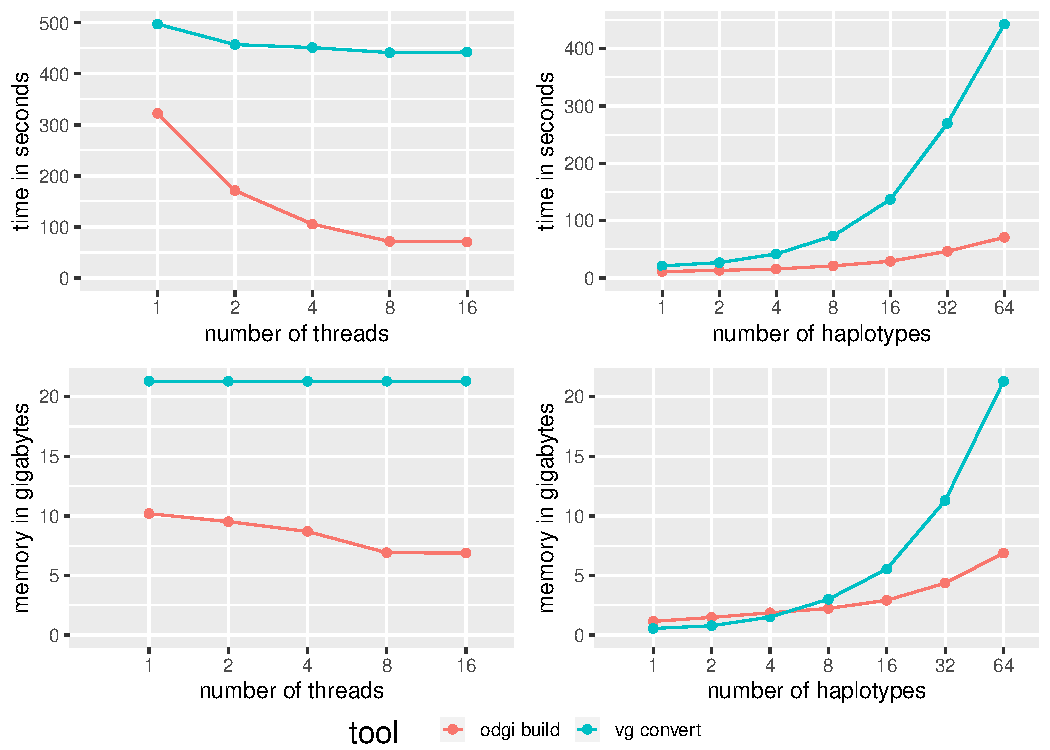
\includegraphics[width=1.0\linewidth, trim=0cm 1.25cm 0cm 0cm]{fig/performance/build_eval.pdf}
		\label{fig:eval-build}
	\end{subfigure}
	\begin{subfigure}{\linewidth}
	\caption{}
	\centering
	% include second image
	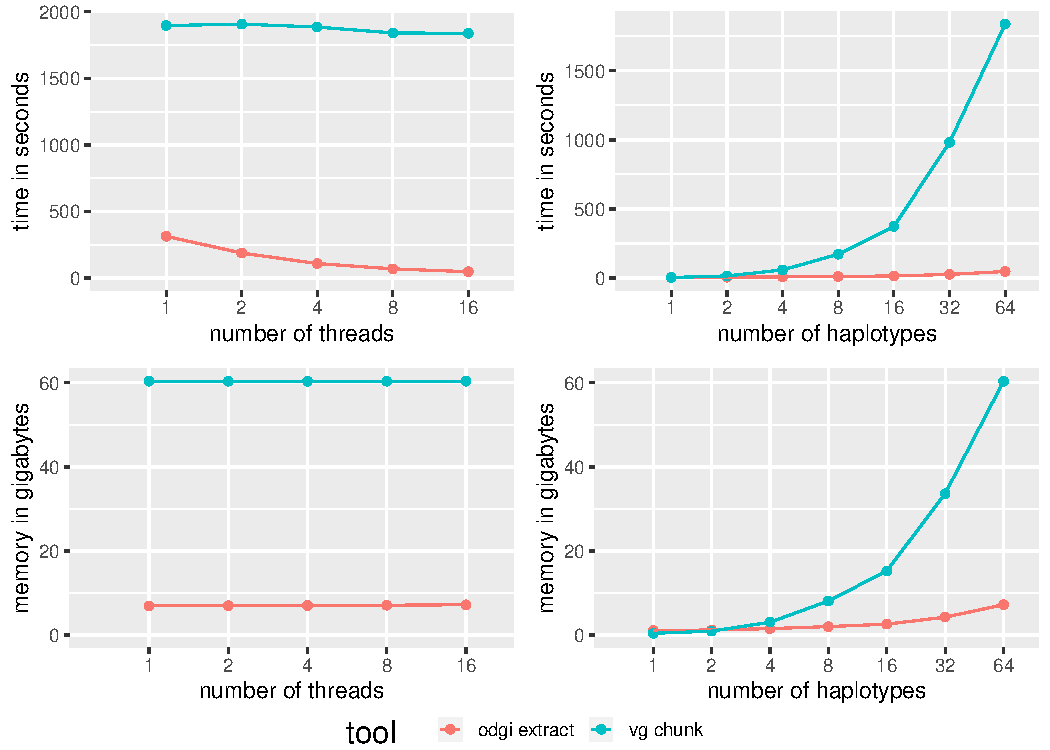
\includegraphics[width=\linewidth, trim=0cm 1.25cm 0cm 0cm]{fig/performance/extract_eval.pdf}
	\label{fig:eval-extract}
	\end{subfigure}
	\begin{subfigure}{1\linewidth}
		\caption{}
		\centering
		% include fourth image
		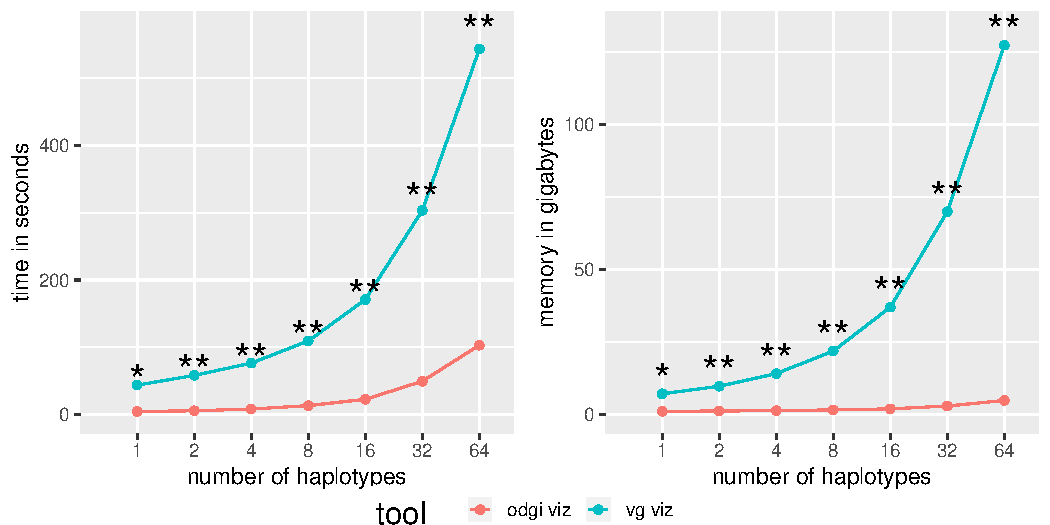
\includegraphics[width=\linewidth, trim=0cm 1.25cm 0cm 0cm]{fig/performance/viz_eval.pdf}
		\label{fig:eval-viz}
	\end{subfigure}
	\caption{\REVIEWED{Performance on a graph of human chromosome 6 from the HPRC. ODGI compares favorably to VG across all routine pangenomic tasks. Evaluations across threads were done using a 64 human haplotype graph. Evaluations across haplotypes were done using 16 threads. \textbf{(a)} Performance evaluation when translating a graph into the tools' respective native formats. \textbf{(b)} Performance evaluation when extracting the centromeric region from the HPRC graph. \textbf{(c)} Performance evaluation when visualizing a graph. Both tools were run with only one thread. \textit{vg viz}: \textbf{*}A 816MB SVG was produced which can't be opened by any program. \textbf{**}All produced SVGs only contain an XML header, nothing else.}}
	\label{fig:evaluation}
\end{figure}


%\begin{figure}[ht!]
	\begin{subfigure}{\linewidth}
		\caption{}
		\centering
		% include second image
		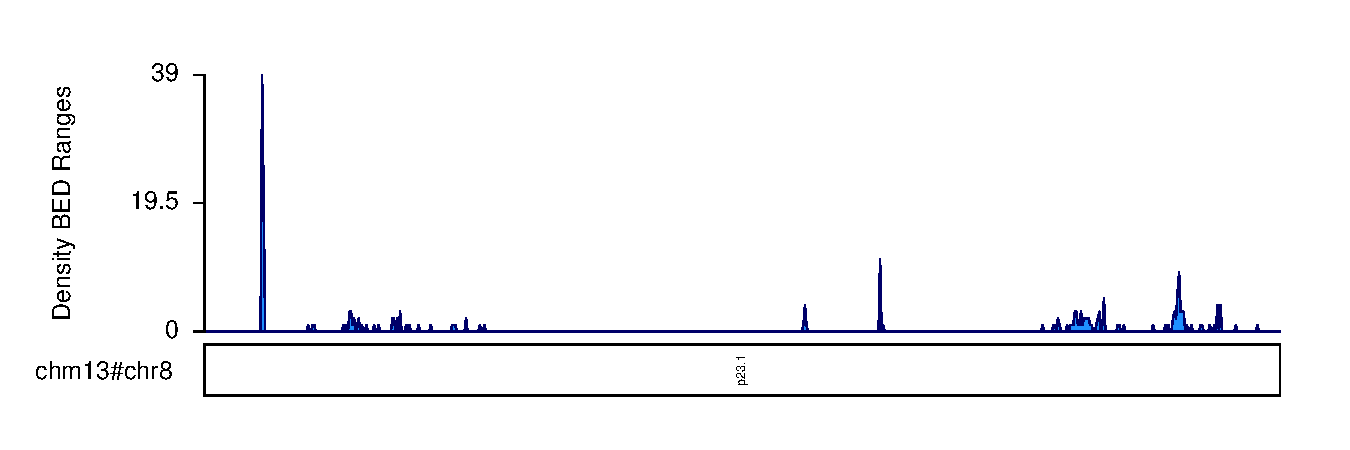
\includegraphics[width=1.0\linewidth, trim=0cm 2.75cm 0cm 0cm]{fig/tips/chr8_chm13_beta_defensin_locus_odgi_tips_w50000_karyoploteR}
		\label{fig:tips-karyo}
	\end{subfigure}
	%	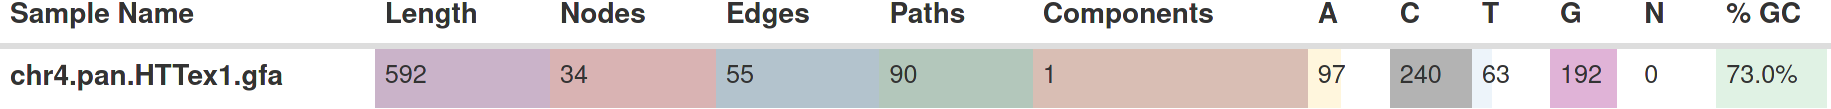
\includegraphics[width=\linewidth]{fig/metrics/chr4.pan.HTTex1.gfa.multiqc_odgi_stats.png}
	\caption{Visualizing the contigs of a beta-defensin locus pangenome graph. (\textbf{a}) Breakpoint ranges of the contigs in the beta-defensin locus pangenome graph of 90 haplotypes relative to CHM13. The \textit{odgi tips} results are visualized as the density of BED ranges across the whole \textit{p23.1} cytoband. The high peak at the beginning of \textit{p23.1} indicates that 39 contigs of the graph broke there relative to CHM13. (\textbf{b}) \FIXME{ADD VIZ AS SOON AS THE SORTING IS FINISHED.}}
	\label{fig:tips}
\end{figure}




% Figure: small graph with all the stats shown. A screenshot of MultiQC, visualize summary per bin somehow, R visualizations of degree and depth HTT exon 1 as tiny example graph

\section{Discussion}
Pangenome graphs stand to become a ubiquitous model in genomics thanks to their capability to represent any genetic variant without being affected by reference bias~\citep{Eizenga_2020}.
However, despite this great potential, their spread is impeded by the lack of tools capable of managing and analyzing pangenome graphs easily and efficiently.

\REVIEWED{By providing a set of standard analysis ``verbs'' to interact with pangenome graphs, ODGI enables users to explore and discover important biological features captured in this flexible, inclusive model.}
It provides tools to easily transform, analyze, simplify, validate, and visualize pangenome graphs at large scale.
In particular, lifting over annotations and linearizing nested graph structures place the suite as the bridge between traditional linear reference genome analysis and pangenome graphs.
With the increased adoption of long read sequencing we expect pangenomic tools to become increasingly common in \REVIEWED{the genomic studies at different taxonomic levels and} in biomedical research.
This progression is already afoot, particularly for targets that involve complex variation, such as cancer\REVIEWED{~\citep{CompPan2016}}, plant pangenomics\REVIEWED{~\citep{Bayer2020, Liu2020, Qin2021, Li2022, Bayer2022}}, and metagenomics\REVIEWED{~\citep{Zhong2021}}. \REVIEWED{Also, when studying animals like bovines~\citep{Leonard2021, Talenti2022, BPC}.}

\REVIEWED{Currently, bacterial pangenomes are best handled by specialized tools like PPanGGolin~\citep{Gautreau2020}, PanGraph~\citep{Noll2022} or PanX~\citep{Wei2017}. The latter one doesn't build a graphical representation of  a pangenome. But, it already has a very developed eco-system, which allows a detailed analysis of bacterial pangenomes using an interactive GUI.
Unlike these approaches, which provide a monolithic, integrated solution to understanding pangenomes, ODGI is designed as a low-level toolkit that can work on a generic pangenome graph model frequently used by other existing methods.
We hope that this design renders it useful to pangenome analysis pipeline authors.
%but it can serve as a strong basis to explore viral and bacterial pangenomes on a very large scale.
Other pangenome analysis platforms, like PanTools~\citep{Sheikhizadeh_2016} provide access to pangenome analyses at the scales we demonstrate with ODGI, but use specialized de Bruijn graph models to achieve this. In contrast ODGI supports the highly generic variation graph model, which has greater representational power than de Bruijn graphs.}

ODGI will facilitate disentangling,
describing and analyzing a much larger set of variation than previously was possible with tools that depend on short reads and reference genomes.
Furthermore, users can even consider ODGI as a framework, taking advantage of its algorithms to develop new and more advanced tools that work on pangenome graphs,
thus expanding the type of possible pangenomic analyses available to the scientific community.

\REVIEWED{The performance analysis shows that ODGI outperforms VG when handling large, complex pangenome graphs.
%This is a major achievement, because VG's XG data structure is static, compared to ODGI's dynamic graph implementation.
Across the evaluation of key graph operations, ODGI's memory peak was 10GB. This makes it perfectly suited to be run interactively on a recent laptop.
%VG has limitations here.
We expect that ODGI will be able to handle the next phase of the HPRC, a pangenome graph constructed from 300 individuals, without any problems.}

\REVIEWED{While ODGI does not construct graphs from scratch nor is is capable of extending them, it} is already the backbone of the Pangenome Graph Builder pipeline~\citep{pggb}.
Its static, large-scale 1D and 2D visualizations of the pangenome graphs allow an unprecedented high-level perspective on variation in pangenomes, and have also been critical in the development of pangenome graph building methods.  %the underlying structure and any problems in graph construction.
However, an interactive solution that combines the 1D and 2D layout of a graph with annotation and read mapping information across different zoom levels is still missing.
\REVIEWED{Recent interactive pangenome graph browsers are reference-centric~\citep{Beyer2019, Yokoyama2019}, have a limited predefined coordinate system~\citep{Durant2021}}, or focus primarily on 2D representations~\citep{Wick_2015, Gonnella2018}.
Our graph sorting and layout algorithms can provide the foundation for future tools of this type.
We plan to focus on using these learned models to detect structural variation and assembly errors.
%In ODGI, we provide a graph layout algorithm that can become a backbone of such tools, as is already the case for \textit{gfaestus}~\citep{gfaestus} %\footnote{\url{https://github.com/chfi/gfaestus}},
%which currently relies on the \textit{odgi layout} output for its interactive 2D graph visualization.

ODGI has allowed us to explore \textit{context mapping} deconvolution of pangenome graph structures via the path jaccard metric.
This resolves a major conceptual issue that has strongly guided existing algorithms to construct pangenome graphs.
Previously, great efforts have been made to prevent the ``collapse'' of non-orthologous sequences in the graph topology itself~\citep{Li:2020}.
This has been seen as essential to making these new bioinformatic models interpretable.
While our presentation is primarily qualitative, our work demonstrates that we can mitigate this issue by exploiting the pangenome graph not as a static reference, but as a dynamic model of the mutual alignment of many \REVIEWED{genomic sequences}.
Because pangenome graphs can contain complete genomes, we are able to query them to polarize the information they contain in easily-interpretable and reusable pairwise formats that are widely supported in bioinformatics.
ODGI also projects variation graphs into vector and matrix representations that allow the direct application of machine learning and statistical models to the pangenome.
%By providing convenient linearizations and matrix transformations, ODGI also provides an interface for machine learning on pangenomes.
%can be linearized into feature vector or matrix form, and ODGI thus provides a natural interface for machine learning and statistical methods that operate directly on data of this shape.
We expect that ODGI will provide a reference interface between pangenomic and genomic approaches for understanding genome variation.

%To understand this model, we query it using any reference that it contains.

%Our future work will focus on further extensions of this topic.

%Here, we present only qualitative evaluation of this result, but our future work will focus on exploiting this mechanism to simplify and aid the interpretation of large pangenomes.

%ODGI aims to be a reference implementation for many pangenome related operations, thus future work will be focused on multiple directions.
%First, we will expand its metadata capabilities to annotate large pangenome graphs.
%Futhermore, we will improve RDF support for annotation in the in-memory graph~\citep{Yokoyama2020} and allow for federated queries on pangenome graphs.
%Finally, we will explore the addition of support for RNA sequences and proteins to extend the application of pangenomic approaches to other levels in the genetic information flow from DNA to phenotype.





%So far, ODGI has not been applied to graphs build from scWGS~\citep{Zhuo2021} data. Each cell would be represented as a path in the graph, the path depth would be very high.
%As ODGI was designed to deal with the path depth of human pangenome graphs, it remains to be seen, if it will work equally well with scWGS data.

\section*{Acknowledgments}

We thank members of the HPRC Pangenome Working Group for their insightful discussion and feedback, and members of the HPRC production teams for their development of resources used in our exposition.

\section*{Funding}

We gratefully acknowledge support from NIH/NIDA U01DA047638 (EG), NIH/NIGMS R01GM123489 (EG and PP), and NSF PPoSS Award \#2118709 (EG and PP).
SH acknowledges funding from the Central Innovation Programme (ZIM) for SMEs of the Federal Ministry for Economic Affairs and Energy of Germany. SN acknowleges Germany’s Excellence Strategy (CMFI), EXC-2124 and (iFIT) - EXC 2180 – 390900677.
This work was supported by the BMBF-funded de.NBI Cloud within the German Network for Bioinformatics Infrastructure (de.NBI) (031A537B, 031A533A, 031A538A, 031A533B, 031A535A, 031A537C, 031A534A, 031A532B).
\linebreak
\linebreak
\REVIEWED{\textit{Conflict of Interest}: the authors declare no competing interests.}


\section*{Data availability}

%Data used to build human pangenome graphs: \url{https://github.com/human-pangenomics/HPP_Year1_Data_Freeze_v1.0}.
%The graphs we generated the figures from: \url{https://s3-us-west-2.amazonaws.com/human-pangenomics/index.html?prefix=pangenomes/scratch/2021_11_04_pggb_wgg.87/}.
Code and links to data resources used to build this manuscript and its figures, can be found in the paper's public repository: \url{https://github.com/pangenome/odgi-paper}.


\bibliographystyle{natbib}
%\bibliographystyle{achemnat}
%\bibliographystyle{plainnat}
%\bibliographystyle{abbrv}
%\bibliographystyle{bioinformatics}
%
%\bibliographystyle{plain}
%
\bibliography{document}


% \begin{thebibliography}{}

% \bibitem[Bofelli {\it et~al}., 2000]{Boffelli03}
% Bofelli,F., Name2, Name3 (2003) Article title, {\it Journal Name}, {\bf 199}, 133-154.

% \bibitem[Bag {\it et~al}., 2001]{Bag01}
% Bag,M., Name2, Name3 (2001) Article title, {\it Journal Name}, {\bf 99}, 33-54.

% \bibitem[Yoo \textit{et~al}., 2003]{Yoo03}
% Yoo,M.S. \textit{et~al}. (2003) Oxidative stress regulated genes
% in nigral dopaminergic neurnol cell: correlation with the known
% pathology in Parkinson's disease. \textit{Brain Res. Mol. Brain
% Res.}, \textbf{110}(Suppl. 1), 76--84.

% \bibitem[Lehmann, 1986]{Leh86}
% Lehmann,E.L. (1986) Chapter title. \textit{Book Title}. Vol.~1, 2nd edn. Springer-Verlag, New York.

% \bibitem[Crenshaw and Jones, 2003]{Cre03}
% Crenshaw, B.,III, and Jones, W.B.,Jr (2003) The future of clinical
% cancer management: one tumor, one chip. \textit{Bioinformatics},
% doi:10.1093/bioinformatics/btn000.

% \bibitem[Auhtor \textit{et~al}. (2000)]{Aut00}
% Auhtor,A.B. \textit{et~al}. (2000) Chapter title. In Smith, A.C.
% (ed.), \textit{Book Title}, 2nd edn. Publisher, Location, Vol. 1, pp.
% ???--???.

% \bibitem[Bardet, 1920]{Bar20}
% Bardet, G. (1920) Sur un syndrome d'obesite infantile avec
% polydactylie et retinite pigmentaire (contribution a l'etude des
% formes cliniques de l'obesite hypophysaire). PhD Thesis, name of
% institution, Paris, France.

% \end{thebibliography}
\clearpage
\setcounter{page}{1}

\beginsupplement

\section{Supplement}

\subsection{Graph topology visualization}
\label{sec:supp_visualization}
In an \textit{odgi viz} visualization, given a path X traversing two nodes A and B, the corresponding edge is represented by a black line starting from the left or right of node A if this node is traversed in reverse or forward, respectively, by path X;
the black line ends to the left or right of node B if this node is traversed in forward or reverse, respectively, by path X.
Consequently, if two consecutive nodes are linked both in forward, no edge is shown (it would be 0 pixels long, as it would start from the right of the first node and ends to the left of the second one).

\subsection{Graph navigation and untangling}
\label{sec:supp_navigation}
Pangenome graphs can model alignments of many genomes.
With \textit{odgi untangle}, users can extract pairwise alignment information between a given set of ``query'' sequences and a given set of ``target'' sequences (used as references).
While pangenome graphs may contain looping structures that imply many-to-many alignments between the pangenome sequences, these untangled alignments map each segment of the queries to a single segment in the set of targets.
\textit{odgi untangle} first discovers segment boundaries using standard approaches for detecting repeats in sequence graphs~\citep{Pevzner_2004}.
We finally ``untangle'' by finding the target segment that best matches each query segment using the \textit{path jaccard} context mapping model.
%The \textit{path jaccard} concept ensures that the breaking is nucleotide-precise.
Moreover, to obtain base-level precise information on the relationships between the repeated sequences, we can align them by using the pairs of regions that came from the untangling to guide the alignment~\citep{wfmash}.

\textit{odgi tips} can identify the break point positions of the contigs relative to the reference(s) in the graph by walking from the ends of each contig until a reference node is found.
It could be that the reference visits the node several times. Therefore, for each contig range (a tip) \textit{odgi tips} takes a look at each possible reference window and finds the most similar one using the \textit{path jaccard} concept.
The output is a BED file with the best reference hit and position for each of the contigs' ends.

\subsubsection{The GFF liftover}
\label{sec:supp_gff}
A GFF file contains annotations for one or more paths in the graph. For each annotation, we know the start and end within that path. So we can annotate all nodes that are visited by such a path range with the information from the attribute field. If there are overlapping features, we append the annotation for each node. Using the same coloring schema as in \textit{odgi viz} we generate a color for each annotated node by its collected annotation.

If a subgraph was as a result from e.g. \textit{odgi extract}, the path names are usually in the form of name:start-end. \textit{odgi position} is able to automatically detect this and adjust the positions given in the GFF on the fly to the new positions given in the subgraph. For each GFF entry, it just subtracts the “missing” number of nucleotides from the start and end field. That’s how we adjust for the subgraph annotation.

\subsubsection{Path Jaccard concept}
\label{sec:supp_path_jaccard}
\textit{odgi tips}, \textit{odgi untangle}, and \textit{odgi position} all translate a query path position to a target path position. In a repeat region, it could be that the node of the query path position ($N_q$) is visited several times by the target path. We use the graph \textit{path jaccard} concept to infer the best target position for a given query path position. For the query position we look at each possible target window and find the most-similar one: 
\begin{enumerate}
	\item~Starting from $N_q$ we follow the steps of one target path position a certain nucleotide distance to the left and a certain nucleotide distance to the right, also called context. The ODGI default distance is 10kbp for each direction.
	\item~We collect all node identifiers that are visited this way in a multi-set.
	\item~Repeat the same process when following the query path position steps.
\end{enumerate}
Now we have two multi-sets of node identifiers, the target path position $T$ one, and the query path position $Q$ one. We apply the Jaccard measure to estimate the similarity between these two multi-sets (Equ.~\ref{eq:jaccard}).
\begin{equation}
	J(T,Q)=\frac{|T\cap Q|}{|T\cup Q|}
	\label{eq:jaccard}
\end{equation}
The "$|$" indicate that, after we joined our sets together, we actually calculate the total length in nucleotides represented by the intersection node set in the nominator, and by the union node set in the denominator, respectively. The division of the two nucleotide lengths then gives us the jaccard measure for the two path positions.
We collect these jaccard measurements for all possible target path positions. The largest \textit{path jaccard} determines the actual target path position for the translation.

Dependent on how repeat-streaked the graph is and how it was constructed, one might want to adjust context size, to get an even more precise positional translation. If we can't follow the full distance to one direction, because we are at an end of a sequence, we also adjust this for all other context evaluating windows.

In the following an example which is based on the graph in Figure~\ref{fig:jaccard}.
\begin{figure}[ht!]
	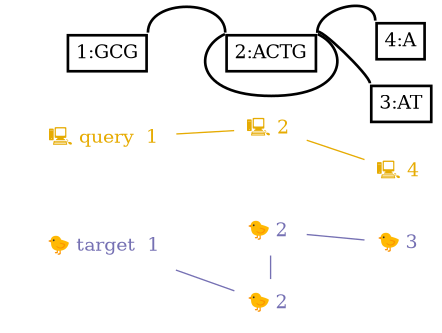
\includegraphics[width=1.0\linewidth]{fig/jaccard/jaccard.png}
	\caption{Simple example graph to demonstrate the \textit{path jaccard} concept. Generated with \textit{vg view} and \textit{graphviz'} \textit{dot} command. On top are the nodes connected with edges. On the bottom the paths through the nodes. Each path has a different color and emoji.}
	\label{fig:jaccard}
\end{figure}
Let's assume, we want to translate the query path position \textit{query:3} to a path position in path \textit{target} with a context distance of 2 nucleotides per direction. Node \textit{2} is where \textit{query:3} is located. The node is traversed two times by \textit{target}. Therefore, we apply the \textit{path jaccard} concept to do a precise position translation. Starting from node \textit{2}, we collect nodes $\{1,2,4\}$ for path \textit{query}. For path \textit{target} we have two possible steps to start our collection from: The first or the second step in node \textit{2}. We obtain the node sets $T_1=\{1,2,2\}$ and $T_2=\{2,2,3\}$.
\begin{multline}
	J_1(T_1,Q)=\frac{|T_1\cap Q|}{|T_1\cup Q|}=\frac{|\{1,2,2\}\cap \{1,2,4\}|}{|\{1,2,2\}\cup \{1,2,4\}|}\\=\frac{|\{1,2\}|}{|\{1,2,2,4\}|}\widehat{=}\frac{3+4}{3+4+4+1}\approx0.58
	\label{eq:jaccard_t1}
\end{multline}
\begin{multline}
	J_2(T_2,Q)=\frac{|T_2\cap Q|}{|T_2\cup Q|}=\frac{|\{2,2,3\}\cap \{1,2,4\}|}{|\{2,2,3\}\cup \{1,2,4\}|}\\=\frac{|\{2\}|}{|\{1,2,2,3,4\}|}\widehat{=}\frac{4}{3+4+4+2+1}\approx0.29
	\label{eq:jaccard_t2}
\end{multline}
We observe a \textit{path jaccard} of $0.58$ for $T_1/Q$ (Equ.~\ref{eq:jaccard_t1}) and $0.29$ for $T_2/Q$ (Equ.~\ref{eq:jaccard_t2}).
Therefore, we translate query path position \textit{query:3} to the target path position \textit{target:3}.

\subsection{Editing}
\label{sec:supp_edit}
Subgraphs can be extracted by using the paths in the graph as coordinate systems to guide the process. For such operation, \textit{odgi extract} allows users to extract specific regions of the graph as defined by query criteria.
Regions of interest can be specified by graph nodes or path range(s), also in BED format. Furthermore, it is possible to indicate a list of paths to be preserved completely in the extracted graph.
We begin by collecting all graph nodes that fall within the ranges to extract (and the paths to preserve, if requested).
Users can specify the number of steps or nucleotides to expand the selection and include neighboring nodes.
Then, edges connecting all selected nodes are added in the subgraph under construction.
Finally, the portions of the paths (i.e., the subpaths) walking through the selected nodes are extracted and added to the new subgraph.
Subpaths are searched in parallel, created serially, and extended in parallel again thanks to the parallelism enabled by the ODGI data structure (see \S\ref{sec:build}), making \textit{odgi extract} a scalable solution to extract also complex subregions presenting nodes with very high node depth.

Pangenome graphs can embed multiple chromosomes as separated connected components (inter-chromosomal structural variants would join the components into bigger ones).
\textit{odgi explode} separates the connected components in different ODGI format files, while \textit{odgi squeeze} allows merging multiple graphs into the same ODGI format file, preventing node ID collisions.

Pangenome graphs can be used in a variety of applications, ranging from read mapping to variant identification and genotyping~\citep{Eizenga_2020}.
However, graphs presenting complex topology can increase the computational overhead of many downstream analyses.
ODGI offers multiple commonly-needed basic operations on the topology of the graph and its nodes.

For simplifying the graph structure, users can use \textit{odgi prune} to take away complex parts as defined by query criteria,
while with \textit{odgi break} they can remove cycles in the graph, reducing the complexity of the graph topology.
Furthermore, \textit{odgi groom} allows removing spurious inverting links by exploring the graph from the orientation supported by most paths;
the process does not remove any genetic information, but only edits how the sequences are represented in the graph.

To enable efficient sequence alignment against the graph, long nodes can be divided into shorter nodes at a maximum requested size using \textit{odgi chop}.
Partial order alignment, which consists of aligning sequences against a directed acyclic graph (DAG), is frequently used in pangenome building pipelines~\citep{pggb}, but the current implementations return DAGs with 1-bp long nodes.
\textit{odgi unchop} allows joining nodes that can be merged without changing the graph topology, nor the embedded sequences, obtaining an equivalent, but more compact, representation of the graph.

\subsection{Sorting and node identifier compaction}
\label{sec:supp_sorting}
Most subcommands in ODGI require and verify that the input graph’s node identifiers (IDs) are optimized, that is compacted from 1 to N where N is the number of nodes in the graph. 
If this assumption is violated, \textit{odgi sort} provides functionality to optimize the graph. 
This means that the first node identifier (ID) starts at 1 and the last node ID is the number of nodes. 
All sorting operations update the graph in place with an efficient ID rewriting algorithm.
The graph is then updated in place. 
First, the node identifiers are normalized (from 1 to number of nodes) including the adjustment of the edges. 
Second, path information, including both path metadata that points into the start and end steps of the path, plus each step of every path, is updated, too. 
We point out that changing the node order does not change our coordinate systems based on paths. 
These will now refer to a new node ordering.

When we sort a graph, we switch the node IDs of the nodes according to the result of the sorting algorithm. 
For example, if a random sort was applied, all existing node IDs would be replaced with new, random ones (the largest node ID would still correspond to the number of nodes on the graph).
We would update the edge and path information as described in the paragraph above.
The reordering of nodes has a great influence on how the pangenome looks like (Fig.~\ref{fig:sorting}).

\begin{figure}[h!]
	\begin{subfigure}{\linewidth}
		%\caption{}
		\centering
		% include first image
		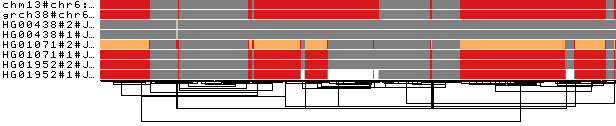
\includegraphics[width=1.0\linewidth, trim=-0cm 2cm 0 0cm]{fig/sorting/chr6_pan_fa_a2fb268_4030258_6a1ecc2_smooth_C4_bad_sorted}
		\label{fig:bad-sorting}
	\end{subfigure}
%	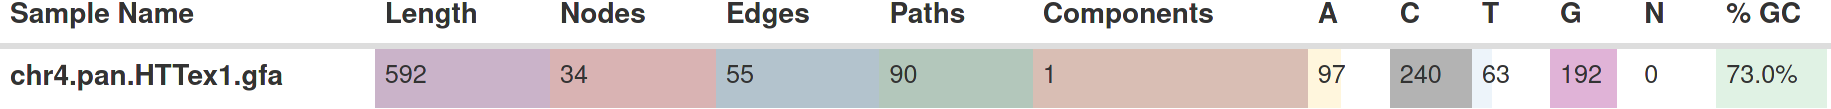
\includegraphics[width=\linewidth]{fig/metrics/chr4.pan.HTTex1.gfa.multiqc_odgi_stats.png}
	\caption{
		Visualization of a poorly sorted C4 pangenome graph.
		Same \textit{odgi viz} visualization as the one shown in Fig.~\ref{fig:odgi_viz}\textbf{e}, but with a graph where the bad node order hides the underlying copy number variation status present in the C4 region.
	}
	\label{fig:sorting}
\end{figure}


\subsection{Linear projections}
\label{sec:supp_metrics}
Pangenome graph topology can be derived by applying \textit{odgi matrix}, obtaining information on graph nodes connections in textual sparse matrix format.
To investigate on the genomic sequences encoded in the graph, \textit{odgi paths} allows users to calculate pairwise overlap statistics of groupings of paths and emit all path sequences in FASTA format, and it also allows the generation of a ``pangenome matrix'' that reports the copy number (presence/absence) of each path over each node.

In standard practice, pangenome analysis examines presence-absence variations (PAVs), which correspond to loci that are present in some samples but not others.
\textit{odgi pav} uses a set of genomic intervals (in BED expressed in the coordinate space of paths in the graph) to demarcate PAVs.
It then describes the coverage of all paths relative to these PAVs, yielding matrix or tabular representation.
The precise determination of PAVs based on graph topology remains an open problem, but practically any method capable of generating a BED file can be used here.
This lets us define PAVs using repeat or gene annotations of the genomes represented as paths in the graph.
A simple technique is to take the output of \textit{odgi flatten}, which generates a linearization of the graph by emitting the pangenome sequence (the concatenation of all node sequences) in FASTA format, and the projection of all paths on the linearized sequence in BED format relative to the graph's paths.

ODGI also supports an experimental binned representation of graphs designed to support the study and visualization of pangenomes at different scales of resolution.
\textit{odgi bin} summarizes graph path information into bins of a specified size, generating a summarized view of gigabase scale graphs in TSV or JSON file formats.
We have further supported this binning approach in pangenome graph ontology model~\citep{Yokoyama2020}. %maybe we want to save this up for the discussion

\clearpage
\subsection{Evaluation}
\begin{table}[!ht]
	\centering
	\ra{1.3}
	\caption{\label{tab:build} Performance measurements when transforming a graph of human chromosome 6 from the HPRC into the tool's native format. \textbf{haps} is the number of haplotypes in the graph. Displayed are the mean results after 10 runs.}
	\begin{tabular}{@{}SSSSSS@{}}
		& & \multicolumn{2}{c}{$\mathbf{time\ in\ seconds}$} & \multicolumn{2}{c}{$\mathbf{memory\ in\ gigabytes}$} \\ \cmidrule(lr){3-4} \cmidrule(lr){5-6}
		{$\mathbf{threads}$} & $\mathbf{haps}$ &{$\mathbf{odgi\ build}$} & {$\mathbf{vg\ convert}$} & {$\mathbf{odgi\ build}$} & $\mathbf{vg\ convert}$ \\ \hline
		1 & 1 & \textbf{10.78} & 21.92 & 1.15 & \textbf{0.56} \\ 
		1 & 2 & \textbf{14.55} & 28.71 & 1.48 & \textbf{0.78} \\ 
		1 & 4 & \textbf{22.28} & 45.02 & 1.82 & \textbf{1.51} \\ 
		1 & 8 & \textbf{43.41} & 78.67 & \textbf{2.52} & 3.01 \\ 
		1 & 16 & \textbf{76.60} & 133.27 & \textbf{3.57} & 5.54 \\ 
		1 & 32 & \textbf{176.55} & 292.32 & \textbf{5.90} & 11.29 \\ 
		1 & 64 & \textbf{322.50} & 497.51 & \textbf{10.19} & 21.3 \\ \midrule
		2 & 1 & \textbf{10.56} & 21.18 & 1.15 & \textbf{0.56} \\ 
		2 & 2 & \textbf{12.79} & 27.51 & 1.48 & \textbf{0.78} \\ 
		2 & 4 & \textbf{17.08} & 43.64 & 1.81 & \textbf{1.51} \\ 
		2 & 8 & \textbf{28.90} & 75.52 & \textbf{2.42} & 3.01 \\ 
		2 & 16 & \textbf{47.93} & 126.71 & \textbf{3.46} & 5.54 \\ 
		2 & 32 & \textbf{102.67} & 280.12 & \textbf{5.58} & 11.29 \\ 
		2 & 64 & \textbf{171.31} & 457.37 & \textbf{9.52} & 21.3 \\ \midrule
		4 & 1 & \textbf{10.54} & 20.69 & 1.15 & \textbf{0.56} \\ 
		4 & 2 & \textbf{12.63} & 27.90 & 1.48 & \textbf{0.78} \\ 
		4 & 4 & \textbf{14.80} & 42.36 & 1.88 & \textbf{1.51} \\ 
		4 & 8 & \textbf{21.00} & 74.80 & \textbf{2.18} & 3.01 \\ 
		4 & 16 & \textbf{32.69} & 123.41 & \textbf{3.08} & 5.54 \\ 
		4 & 32 & \textbf{65.30} & 271.10 & \textbf{4.87} & 11.29 \\ 
		4 & 64 & \textbf{105.51} & 451.54 & \textbf{8.70} & 21.3 \\ \midrule
		8 & 1 & \textbf{11.53} & 20.33 & 1.15 & \textbf{0.56} \\ 
		8 & 2 & \textbf{13.16} & 27.18 & 1.48 & \textbf{0.78} \\ 
		8 & 4 & \textbf{15.61} & 41.77 & 1.85 & \textbf{1.51} \\ 
		8 & 8 & \textbf{19.63} & 73.09 & \textbf{2.20} & 3.01 \\ 
		8 & 16 & \textbf{28.43} & 131.82 & \textbf{2.87} & 5.54 \\ 
		8 & 32 & \textbf{46.23} & 256.74 & \textbf{4.30} & 11.29 \\ 
		8 & 64 & \textbf{71.55} & 441.59 & \textbf{6.91} & 21.30 \\ \midrule
		16 & 1 & \textbf{11.18} & 21.14 & 1.15 & \textbf{0.56} \\ 
		16 & 2 & \textbf{13.27} & 26.74 & 1.48 & \textbf{0.78} \\ 
		16 & 4 & \textbf{15.55} & 41.90 & 1.87 & \textbf{1.51} \\ 
		16 & 8 & \textbf{21.16} & 73.36 & \textbf{2.24} & 3.01 \\ 
		16 & 16 & \textbf{29.09} & 136.96 & \textbf{2.92} & 5.54 \\ 
		16 & 32 & \textbf{46.58} & 269.61 & \textbf{4.36} & 11.29 \\ 
		16 & 64 & \textbf{70.84} & 442.71 & \textbf{6.89} & 21.30 \\ \bottomrule
	\end{tabular}
\end{table}
\clearpage
\begin{table}[!ht]
	\centering
	\ra{1.3}
	\caption{\label{tab:extract} Performance measurements when extracting the centromeric region of a human chromosome 6 pangenome graph. \textbf{haps} is the number of haplotypes in the graph. Displayed are the mean results after 10 runs.}
	\begin{tabular}{@{}SSSSSS@{}}
		& & \multicolumn{2}{c}{$\mathbf{time\ in\ seconds}$} & \multicolumn{2}{c}{$\mathbf{memory\ in\ gigabytes}$} \\ \cmidrule(lr){3-4} \cmidrule(lr){5-6}
		{$\mathbf{threads}$} & {$\mathbf{haps}$} & {$\mathbf{odgi\ extract}$} & {$\mathbf{vg\ chunk}$} & {$\mathbf{odgi\ extract}$} & {$\mathbf{vg\ chunk}$} \\ \hline
		1 & 1 & 3.65 & \textbf{3.34} & 1.07 & \textbf{0.42} \\ 
		1 & 2 & \textbf{6.08} & 14.25 & 1.22 & \textbf{0.95} \\ 
		1 & 4 & \textbf{15.96} & 58.67 & \textbf{1.51} & 3.06 \\ 
		1 & 8 & \textbf{37.16} & 170.63 & \textbf{1.91} & 8.12 \\ 
		1 & 16 & \textbf{67.47} & 364.98 & \textbf{2.49} & 15.25 \\ 
		1 & 32 & \textbf{161.32} & 968.71 & \textbf{4.00} & 33.65 \\ 
		1 & 64 & \textbf{313.05} & 1897.00 & \textbf{6.96} & 60.37 \\ \midrule
		2 & 1 & 3.67 & \textbf{3.33} & 1.07 & \textbf{0.42} \\ 
		2 & 2 & \textbf{5.50} & 13.57 & 1.22 & \textbf{0.96} \\ 
		2 & 4 & \textbf{12.33} & 56.44 & \textbf{1.51} & 3.06 \\ 
		2 & 8 & \textbf{24.06} & 170.62 & \textbf{1.92} & 8.12 \\ 
		2 & 16 & \textbf{43.49} & 376.67 & \textbf{2.51} & 15.25 \\ 
		2 & 32 & \textbf{97.03} & 987.85 & \textbf{4.03} & 33.65 \\ 
		2 & 64 & \textbf{187.51} & 1907.98 & \textbf{7.00} & 60.37 \\ \midrule
		4 & 1 & 3.64 & \textbf{3.32} & 1.07 & \textbf{0.42} \\ 
		4 & 2 & \textbf{5.59} & 13.40 & 1.22 & \textbf{0.96} \\ 
		4 & 4 & \textbf{9.93} & 57.67 & \textbf{1.52} & 3.06 \\ 
		4 & 8 & \textbf{16.58} & 174.94 & \textbf{1.94} & 8.11 \\ 
		4 & 16 & \textbf{27.99} & 374.99 & \textbf{2.52} & 15.26 \\ 
		4 & 32 & \textbf{56.94} & 992.85 & \textbf{4.06} & 33.65 \\ 
		4 & 64 & \textbf{108.34} & 1885.91 & \textbf{7.04} & 60.37 \\ \midrule
		8 & 1 & 3.61 & \textbf{3.30} & 1.07 & \textbf{0.42} \\ 
		8 & 2 & \textbf{5.47} & 14.01 & 1.22 & \textbf{0.96} \\ 
		8 & 4 & \textbf{8.43} & 58.69 & \textbf{1.53} & 3.06 \\ 
		8 & 8 & \textbf{12.40} & 180.51 & \textbf{1.98} & 8.11 \\ 
		8 & 16 & \textbf{19.11} & 379.25 & \textbf{2.55} & 15.26 \\ 
		8 & 32 & \textbf{36.35} & 991.09 & \textbf{4.11} & 33.65 \\ 
		8 & 64 & \textbf{68.54} & 1841.57 & \textbf{7.11} & 60.37 \\ \midrule
		16 & 1 & 3.64 & \textbf{3.34} & 1.07 & \textbf{0.42} \\ 
		16 & 2 & \textbf{5.53} & 14.67 & 1.22 & \textbf{0.95} \\ 
		16 & 4 & \textbf{7.62} & 58.22 & \textbf{1.54} & 3.06 \\ 
		16 & 8 & \textbf{10.55} & 171.90 & \textbf{2.03} & 8.12 \\ 
		16 & 16 & \textbf{14.80} & 373.70 & \textbf{2.60} & 15.26 \\ 
		16 & 32 & \textbf{25.51} & 981.79 & \textbf{4.27} & 33.65 \\ 
		16 & 64 & \textbf{46.87} & 1838.51 & \textbf{7.23} & 60.37 \\ \bottomrule
	\end{tabular}
\end{table}
\clearpage
\begin{table}[!ht]
	\centering
	\ra{1.2}
	\caption{\label{tab:viz} Performance measurements when visualizing a human chromosome 6 pangenome graph. \textbf{haps} is the number of haplotypes in the graph. Both \textit{odgi viz} and \textit{vg viz} were run with 1 thread. Displayed are the mean results after 10 runs. \textbf{*}A 816MB SVG was produced which can't be opened by any program. \textbf{**}All produced SVGs were empty except for an XML header.}
	\begin{tabular}{@{}SSSSS@{}}
		& \multicolumn{2}{c}{$\mathbf{time\ in\ seconds}$} & \multicolumn{2}{c}{$\mathbf{memory\ in\ gigabytes}$} \\ \cmidrule(lr){2-3} \cmidrule(lr){4-5}
		{$\mathbf{haps}$} & {$\mathbf{odgi\ viz}$} & {$\mathbf{vg\ viz}$} & {$\mathbf{odgi\ viz}$} & {$\mathbf{vg\ viz}$} \\ \hline
		1 & \textbf{4.14} & 43.40\ \ * & \textbf{1.04} & 7.09\ \ * \\ 
		2 & \textbf{5.30} & 57.94\ \ ** & \textbf{1.14} & 9.69\ \ ** \\ 
		4 & \textbf{7.85} & 76.15\ \ ** & \textbf{1.27} & 14.05\ \ ** \\ 
		8 & \textbf{12.95} & 109.16** & \textbf{1.53} & 21.84\ \ ** \\ 
		16 & \textbf{22.33} & 170.72** & \textbf{1.88} & 36.97\ \ ** \\ 
		32 & \textbf{49.24} & 303.40** & \textbf{2.87} & 69.88\ \ ** \\ 
		64 & \textbf{102.82} & 543.50** & \textbf{4.78} & 127.36** \\ \bottomrule
	\end{tabular}
\end{table}
\clearpage
\begin{table}[!ht]
	\centering
	\ra{1.3}
	\caption{\label{tab:position} Performance measurements when locating all path positions of a node in a human chromosome 6 pangenome graph. \textbf{haps} is the number of haplotypes in the graph. Displayed are the mean results after 10 runs. The number of threads does not affect the running time or memory consumption. \textit{vg find} had to be run for each path position. The total run time of finding all path positions of a node is reported here.}
	\begin{tabular}{@{}SSSSSS@{}}
		& & \multicolumn{2}{c}{$\mathbf{time\ in\ seconds}$} & \multicolumn{2}{c}{$\mathbf{memory\ in\ gigabytes}$} \\ \cmidrule(lr){3-4} \cmidrule(lr){5-6}
		{$\mathbf{threads}$} & {$\mathbf{haps}$} & {$\mathbf{odgi\ position}$} & {$\mathbf{vg\ find}$} & {$\mathbf{odgi\ position}$} & {$\mathbf{vg\ find}$} \\ \hline
		1 & 1 & 2.58 & \textbf{0.16} & 1.01 & \textbf{0.21} \\ 
		1 & 2 & 3.19 & \textbf{0.39} & 1.11 & \textbf{0.26} \\ 
		1 & 4 & 3.52 & \textbf{1.23} & 1.23 & \textbf{0.42} \\ 
		1 & 8 & \textbf{3.97} & 4.28 & 1.49 & \textbf{0.74} \\ 
		1 & 16 & \textbf{5.07} & 14.32 & 1.81 & \textbf{1.25} \\ 
		1 & 32 & \textbf{7.79} & 55.61 & 2.73 & \textbf{2.46} \\ 
		1 & 64 & \textbf{15.60} & 198.54 & \textbf{4.51} & 4.56 \\ \midrule
		2 & 1 & 2.54 & \textbf{0.16} & 1.01 & \textbf{0.21} \\ 
		2 & 2 & 3.17 & \textbf{0.38} & 1.11 & \textbf{0.26} \\ 
		2 & 4 & 3.55 & \textbf{1.24} & 1.23 & \textbf{0.42} \\ 
		2 & 8 & \textbf{3.95} & 4.31 & 1.49 & \textbf{0.74} \\ 
		2 & 16 & \textbf{5.08} & 14.10 & 1.81 & \textbf{1.25} \\ 
		2 & 32 & \textbf{7.76} & 55.56 & 2.73 & \textbf{2.46} \\ 
		2 & 64 & \textbf{15.34} & 198.56 & \textbf{4.51} & 4.56 \\ \midrule
		4 & 1 & 2.67 & \textbf{0.16} & 1.01 & \textbf{0.21} \\ 
		4 & 2 & 3.15 & \textbf{0.38} & 1.11 & \textbf{0.26} \\ 
		4 & 4 & 3.55 & \textbf{1.23} & 1.23 & \textbf{0.42} \\ 
		4 & 8 & \textbf{3.98} & 4.31 & 1.49 & \textbf{0.74} \\ 
		4 & 16 & \textbf{5.06} & 14.23 & 1.81 & \textbf{1.25} \\ 
		4 & 32 & \textbf{7.79} & 55.66 & 2.73 & \textbf{2.46} \\ 
		4 & 64 & \textbf{15.41} & 196.6 & \textbf{4.51} & 4.56 \\ \midrule
		8 & 1 & 2.59 & \textbf{0.16} & 1.01 & \textbf{0.21} \\ 
		8 & 2 & 3.20 & \textbf{0.38} & 1.11 & \textbf{0.26} \\ 
		8 & 4 & 3.55 & \textbf{1.25} & 1.23 & \textbf{0.42} \\ 
		8 & 8 & \textbf{3.99} & 4.31 & 1.49 & \textbf{0.74} \\ 
		8 & 16 & \textbf{5.07} & 14.20 & 1.81 & \textbf{1.25} \\ 
		8 & 32 & \textbf{7.70} & 55.12 & 2.73 & \textbf{2.46} \\ 
		8 & 64 & \textbf{15.9} & 203.02 & \textbf{4.51} & 4.56 \\ \midrule
		16 & 1 & 2.62 & \textbf{0.16} & 1.01 & \textbf{0.21} \\ 
		16 & 2 & 3.16 & \textbf{0.38} & 1.11 & \textbf{0.26} \\ 
		16 & 4 & 3.55 & \textbf{1.23} & 1.23 & \textbf{0.42} \\ 
		16 & 8 & \textbf{3.95} & 4.26 & 1.49 & \textbf{0.74} \\ 
		16 & 16 & \textbf{5.1} & 14.3 & 1.81 & \textbf{1.25} \\ 
		16 & 32 & \textbf{7.66} & 54.78 & 2.73 & \textbf{2.46} \\ 
		16 & 64 & \textbf{15.5} & 202.57 & \textbf{4.51} & 4.56 \\ \bottomrule
	\end{tabular}
\end{table}
\clearpage
\begin{table}[!ht]
	\centering
	\ra{1.2}
	\caption{\label{tab:disk_space} Disk space measurements of GFAv1 and the respective tools' binary formats. \textbf{haps} is the number of haplotypes in the graph. For VG, the file size of the XG format was measured.}
	\begin{tabular}{@{}rr|rr@{}}
		& \multicolumn{3}{c}{$\mathbf{disk\ space\ in\ megabytes}$} \\ \cmidrule(lr){2-4}
		{$\mathbf{haps}$} & {$\mathbf{GFAv1}$} & {$\mathbf{ODGI}$} & {$\mathbf{VG}$} \\ \hline
		1 & 283 & 604 & \textbf{189} \\ 
		2 & 333 & 660 & \textbf{237} \\ 
		4 & 432 & 745 & \textbf{394} \\ 
		8 & 622 & 968 & \textbf{706} \\ 
		16 & 947 & 1277 & \textbf{1200} \\ 
		32 & 1657 & \textbf{2131} & 2388 \\ 
		64 & 2913 & \textbf{3745} & 4426 \\ \bottomrule
	\end{tabular}
\end{table}


\end{document}
